\documentclass{bmstu}
\bibliography{biblio}
\usepackage{pdfpages}

%\usepackage[backend=biber]

\begin{document}
    \makethesistitle
    {Информатика и системы управления} % Название факультета
    {Программное обеспечение ЭВМ и информационные технологии} % Название кафедры
    {Метод прогнозирования задержки рейсов на основе итеративной адаптации с учётом пространственно--временных факторов} % Тема работы
    {Й.~Н.~Везирова/ИУ7И-81Б} % #7 Автор
    {Ю.~В.~Строганов} % ФИО научного руководителя
    {} % ФИО консультанта (необязательный аргумент; если консультантов несколько, их необходимо разделить запятой)
    {} % ФИО нормоконтролера

    \setcounter{page}{3}

%    \addcontentsline{toc}{chapter}{РЕФЕРАТ}
\chapter*{\makebox[1.0\linewidth]{РЕФЕРАТ}}

Расчетно-пояснительная записка~\pageref{LastPage} с., \totalfigures\ рис., 3 лист., 14 ист., 1 прил.

БАЗА ДАННЫХ, PostgreSQL, CИСТЕМА УПРАВЛЕНИЯ БАЗАМИ ДАННЫХ, Python, SQLAlchemy, РЕЛЯЦИОННАЯ МОДЕЛЬ.

Цель работы: разработка базы данных для прогнозирования вероятности задержки рейса в городе--пересадки из--за технического обслуживания.

Данный курсовой проект включет в себя анализ, проектирование и разработку
базы данных для прогнозирования вероятности задержки рейса в городе--пересадки из--за технического обслуживания.
В качестве системы управления базами данных была выбрана PostgreSQL, а для взаимодействия с базами данных в объектно--ориентированной парадигме была выбрана технология SQLAlchemy с реализацией на языке программирования Python.

На базе результатов анализа были разработаны база данных, хранимая процедура и триггер для работы с базой данных.

\begin{essay}{}
    Ключевые слова: регрессия, линейная регрессия, логистическая регрессия, адаптивная регрессия, анализ данных, прогнозирование, интерпретация, сравнение методов.

    Цель работы --- провести анализ методов и подходов к решению задачи регрессии.

    В данной работе рассматриваются предметная область и существующие подходы к решению задачи регрессии, формулируются критерии сравнения и проводится классификация методов.
    По результатам сравнения представлены выводы о рассматриваемых решениях задачи регрессии.
\end{essay}

\newpage
\addcontentsline{toc}{chapter}{ВВЕДЕНИЕ}
\chapter*{\makebox[1.0\linewidth]{ВВЕДЕНИЕ}}

Воздушные перевозки являются одним из наиболее предпочтительных и быстрых видов транспорта.
Самолеты --- это самые известные средства воздушного транспорта и могут использоваться не только для коммерческих/некоммерческих пассажирских перевозок, но и для транспортировки грузов и оборудования.
Объем коммерческих авиаперевозок непрерывно растет во всем мире на протяжении десятилетий, поэтому для поддержания или улучшения качества сервиса, необходимо удовлетворять ожидания пассажиров.
Поскольку пунктуальность оказывает влияние на предпочтения пассажиров при выборе авиалиний, крайне важно, чтобы рейсы четко придерживались своего расписания~\cite{tat}.

Заблаговременное информирование о вероятности задержки рейса пассажиров позволяет последним принимать более рациональные решения, включая выбор альтернативных маршрутов или распределение времени для учета возможных задержек.
Авиакомпании, в свою очередь, могут использовать такие прогнозы для управления ожиданиями пассажиров и реализации мер по снижению потенциальных негативных воздействий на их путешествия~\cite{trt}.

Целью работы является разработка базы данных для прогнозирования вероятности задержки рейса в городе--пересадки из--за технического обслуживания.

Для достижения цели необходимо выполнить следующие задачи:
\begin{enumerate}[label=\arabic*)]
    \item провести анализ предметной области;
    \item спроектировать и разработать базу данных в соответствии с поставленной задачей;
    \item выбрать средства реализации базы данных и приложения;
    \item провести сравнительный анализ работы со строками в хранимой процедуре.
\end{enumerate}

\chapter*{ВВЕДЕНИЕ}
\addcontentsline{toc}{chapter}{ВВЕДЕНИЕ}

Регрессионный анализ по праву может быть назван основным методом современной математической статистики.
Он стал неотъемлемой частью современных методов анализа данных, находя свое отражение в различных подходах, включая методы усреднения, процедуры сглаживания, алгоритмы согласования противоречивых данных и концепции, основанные на принципах оптимальности.
Регрессия --- это квинтэссенция понятия целесообразности~\cite{norman}.

Решение задачи регрессии является ключевым этапом в анализе данных и активно применяется в самых разнообразных областях: от анализа экономических процессов и прогнозирования рыночных тенденций до моделирования сложных физических и инженерных систем.
Такие методы позволяют учитывать нелинейные зависимости, высокую размерность признаков и наличие выбросов, что делает их универсальным инструментом для обработки и интерпретации сложных данных~\cite{bishop}.

Целью работы является проведение анализа методов и подходов к решению задачи регрессии.

Для достижения поставленной цели, необходимо решить следующие задачи:
\begin{itemize}
    \item провести анализ предметной области;
    \item провести обзор существующих решений задачи регрессии;
    \item сформулировать критерии сравнения решений задачи регрессии;
    \item классифицировать существующие решения задачи регрессии.
\end{itemize}

\chapter{Аналитический раздел}

В данном разделе будет проведен анализ предметной области, существующих решений и формулировка требований к разрабатываемой базе данных.

\section{Анализ предметной области}

Операции по техническому обслуживанию самолетов широко распространены внутри стран и между ними и выполняются как военными, так и гражданскими механиками.
Механики работают в аэропортах, на ремонтных базах, военных объектах.
Механиков нанимают пассажирские и грузовые перевозчики, подрядчики по техническому обслуживанию, сельскохозяйственные предприятия, а также владельцы государственного и частного флота.
Небольшие аэропорты могут обеспечить работой несколько механиков, в то время как в крупных узловых аэропортах и на базах технического обслуживания могут работать тысячи.
Работы по техническому обслуживанию делятся на те, которые необходимы для поддержания текущих повседневных операций (линейное техническое обслуживание), и на те, в процессе которых периодически проверяют, обслуживают и ремонтируют самолет (базовое техническое обслуживание).
Линейное техническое обслуживание включает в себя техническое обслуживание в пути (между посадкой и взлетом) и техническое обслуживание в ночное время.
Техническое обслуживание в пути состоит из эксплуатационных проверок и необходимого в полете ремонта для устранения несоответствий, обнаруженных во время полета.
Этот ремонт, как правило, незначителен, например, замена сигнальных ламп, шин и компонентов авионики, но может быть таким же масштабным, как замена двигателя.
Ночное техническое обслуживание более обширно и включает в себя любой ремонт, отложенный во время дневных полетов.

Сроки, распределение работников и характер технического обслуживания самолетов контролируются каждой авиакомпанией и документируются в ее руководстве по техническому обслуживанию.
Эти плановые мероприятия по техническому обслуживанию обеспечивают проверку, техническое обслуживание и ремонт всего воздушного судна через соответствующие промежутки времени.
Проверки технического обслуживания более низкого уровня могут быть включены в работы по техническому обслуживанию линии, но более обширные работы выполняются на базе технического обслуживания.
Повреждения самолета и отказы компонентов устраняются по мере необходимости~\cite{otplane}.

Время оборота самолета (\textit{англ.} TAT --- turnaround time) --- это общее время, которое требуется для выполнения всех необходимых действий для подготовки самолета к следующему рейсу.
Из--за ограниченного пространства вокруг самолета, операции оборота должны выполняться в точной хронологической последовательности: некоторые из них обязательно должны выполняться последовательно, в то время как другие могут выполняться одновременно.
Эффективность оборота самолета можно определить как способность выполнения необходимых операций в доступное время для обеспечения пунктуального вылета.

Наземное обслуживание самолета --- это сервисный процесс с жесткими требованиями, включающий более 10 взаимосвязанных подпроцессов и вовлекающий более 30 различных сотрудников.

На рисунке~\ref{fig:tat} представлена схема процесса наземного обслуживания самолета, включающая три основные категории обслуживания: пассажиров, багажа и груза, а также самого самолета.

\begin{figure}[h]
    \centering
    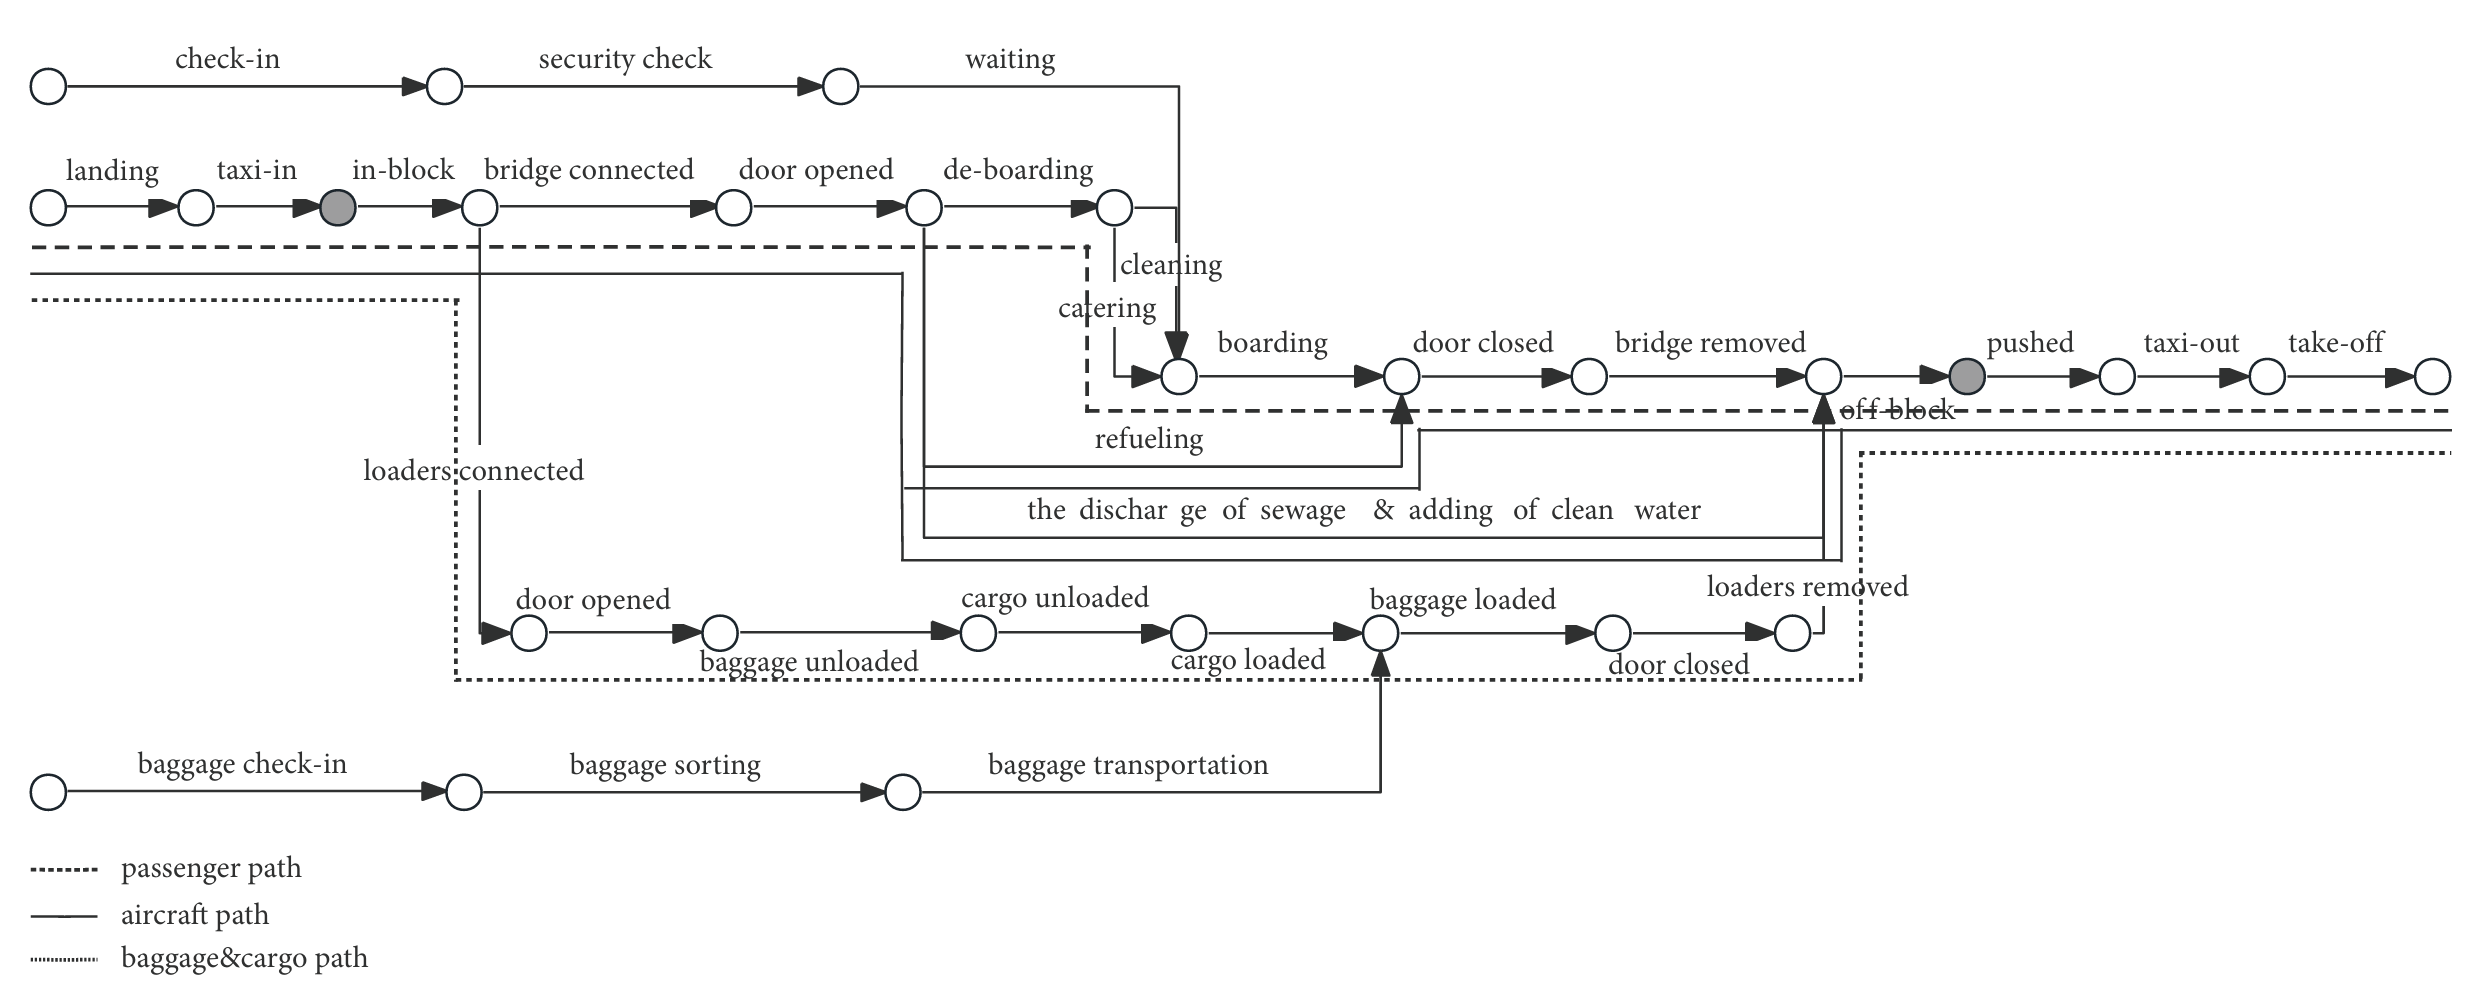
\includegraphics[scale=0.25]{inc/tat}
    \caption{Схема процессов наземного обслуживания самолета}
    \label{fig:tat}
\end{figure}

Пассажиры проходят регистрацию, проверку безопасности и ожидают посадки.
После посадки самолета пассажиры выходят через подключенный мост и проходят высадку.
После уборки и обслуживания питания начинается посадка пассажиров на следующий рейс.

Багаж регистрируется, сортируется и транспортируется к самолету.
После посадки самолета багаж выгружается и новый багаж загружается.
После завершения загрузки багажных отсеков двери закрываются.

Самолет проходит этапы от посадки до взлета, включая такси, подключение моста, открытие дверей, разгрузку и загрузку багажа и груза, заправку, уборку, обслуживание питания и техническое обслуживание.
После завершения всех операций, мост убирается, самолет выталкивается, проходит такси и взлетает.


Эта схема иллюстрирует важность координации и последовательности действий для обеспечения эффективного и своевременного оборота самолета~\cite{trt-timeestimation}.


\section{Анализ существующих решений}

Существует несколько решений в сфере мониторинга полетов, которые обеспечивают отслеживание воздушного движения в реальном времени:
\begin{enumerate}[label=\arabic*)]
    \item Flightradar24 --- это глобальный сервис отслеживания рейсов, который предоставляет информацию о 1000 воздушных судов по всему миру в режиме реального времени~\cite{flightradar24};
    \begin{figure}[h]
        \centering
        \includegraphics[scale=0.1]{inc/flightradar24}
        \caption{Пример отслеживания полетов на Flightradar24}
        \label{fig:flightradar24}
    \end{figure}
    \item FlightAware --- это цифровая авиационная компания, которая управляет крупнейшей в мире платформой отслеживания полетов и сбора данных.
    Благодаря глобальной связи с каждым сегментом авиации, FlightAware предоставляет более 10000 эксплуатантам воздушных судов и поставщикам услуг, а также более 13 000 000 пассажиров глобальные решения для отслеживания полетов, технологии прогнозирования, аналитики и инструменты принятия решений~\cite{flightaware}.
    \begin{figure}[h]
        \centering
        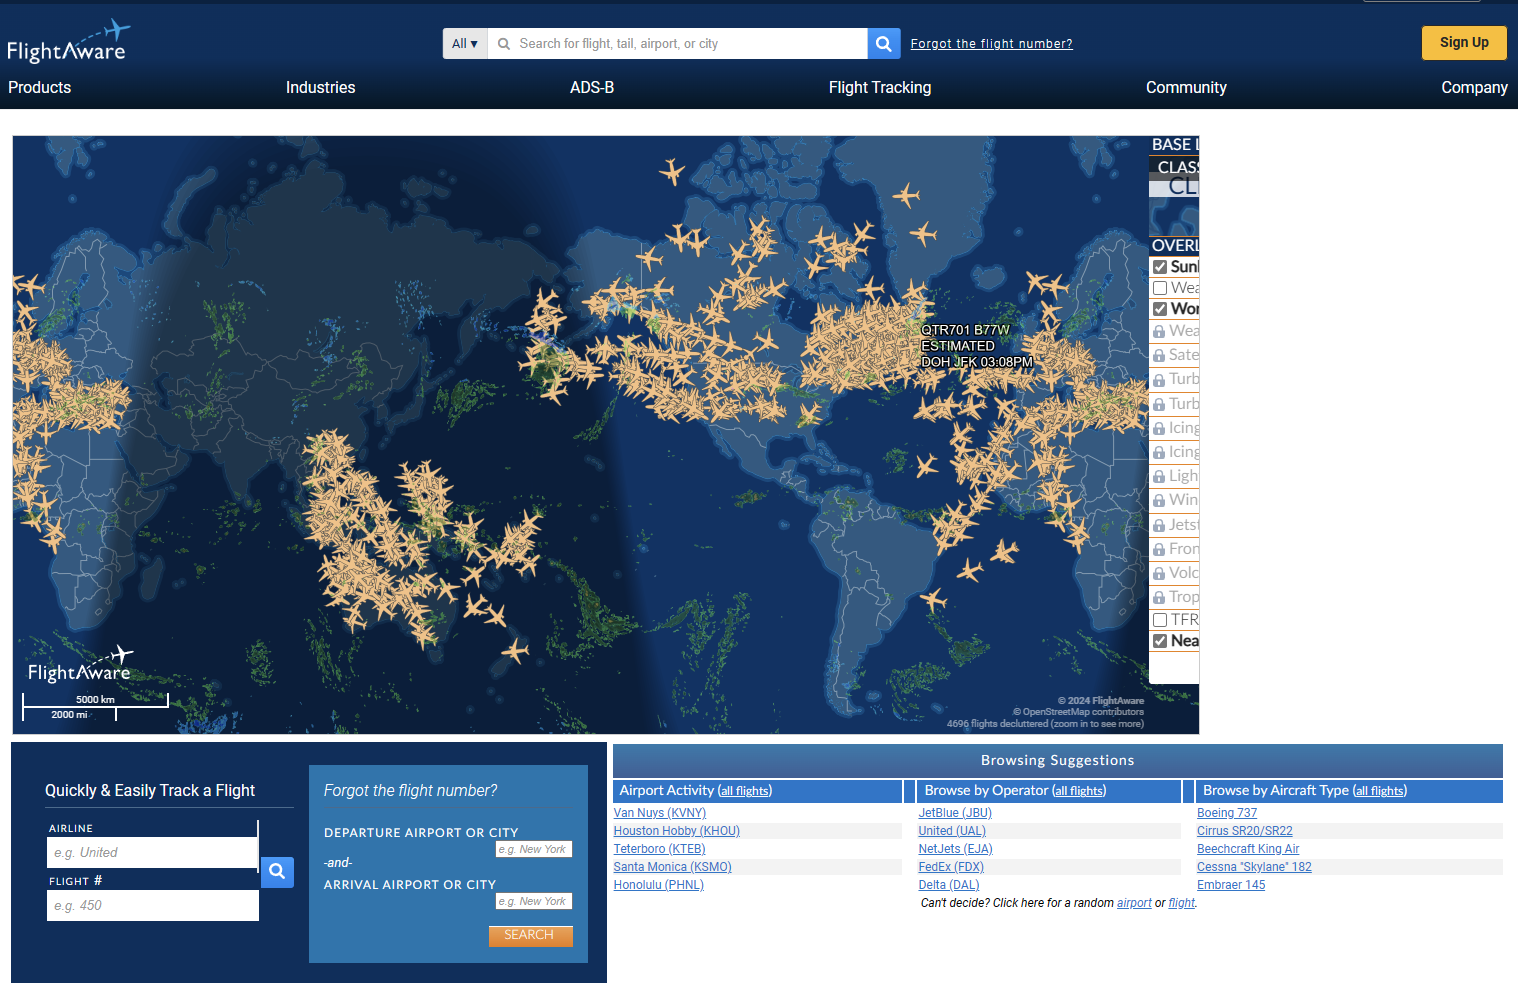
\includegraphics[scale=0.3]{inc/flightaware}
        \caption{Пример отслеживания полетов на FlightAware}
        \label{fig:flightaware}
    \end{figure}
\end{enumerate}


\section{Формализация информации, хранимой в базе данных}

Для наполнения данными базы данных были использованы датасеты с платформы Kaggle, что позволило провести более глубокий анализ полученных результатов.
Это платформа для машинного обучения и аналитики данных, которая предоставляет доступ к множеству датасетов, подготовленных сообществом~\cite{kaggle}.
На платформе Kaggle были найдены датасеты, содержащие информацию о задержках рейсов, аэропортах, авиакомпаниях и полетах.

После анализа датасетов были выделены следующие сущности:
\begin{enumerate}[label=\arabic*)]
    \item полет;
    \item задержка;
    \item аэропорт;
    \item авиакомпания;
    \item самолет;
    \item экипаж;
    \item отчет;
    \item система.
\end{enumerate}

На рисунке~\ref{fig:er} представлена ER--диаграмма сущностей системы в нотации Чена.

\begin{figure}[H]
    \centering
    \includegraphics[scale=0.45]{inc/Drawing1}
    \caption{ER -- диаграмма для базы данных}
    \label{fig:er}
\end{figure}

\section{Система ролей в базе данных}

Ролевая модель в базе данных состоит из трех ролей:
\begin{enumerate}[label=\arabic*)]
    \item гость --- пользователь, у которого есть доступ к чтению сущностей полета, аэропорта, авиакомпании, задержки, а также возможность получить информацию о вероятности задержки конкретного перелета;
    \begin{figure}[H]
        \centering
        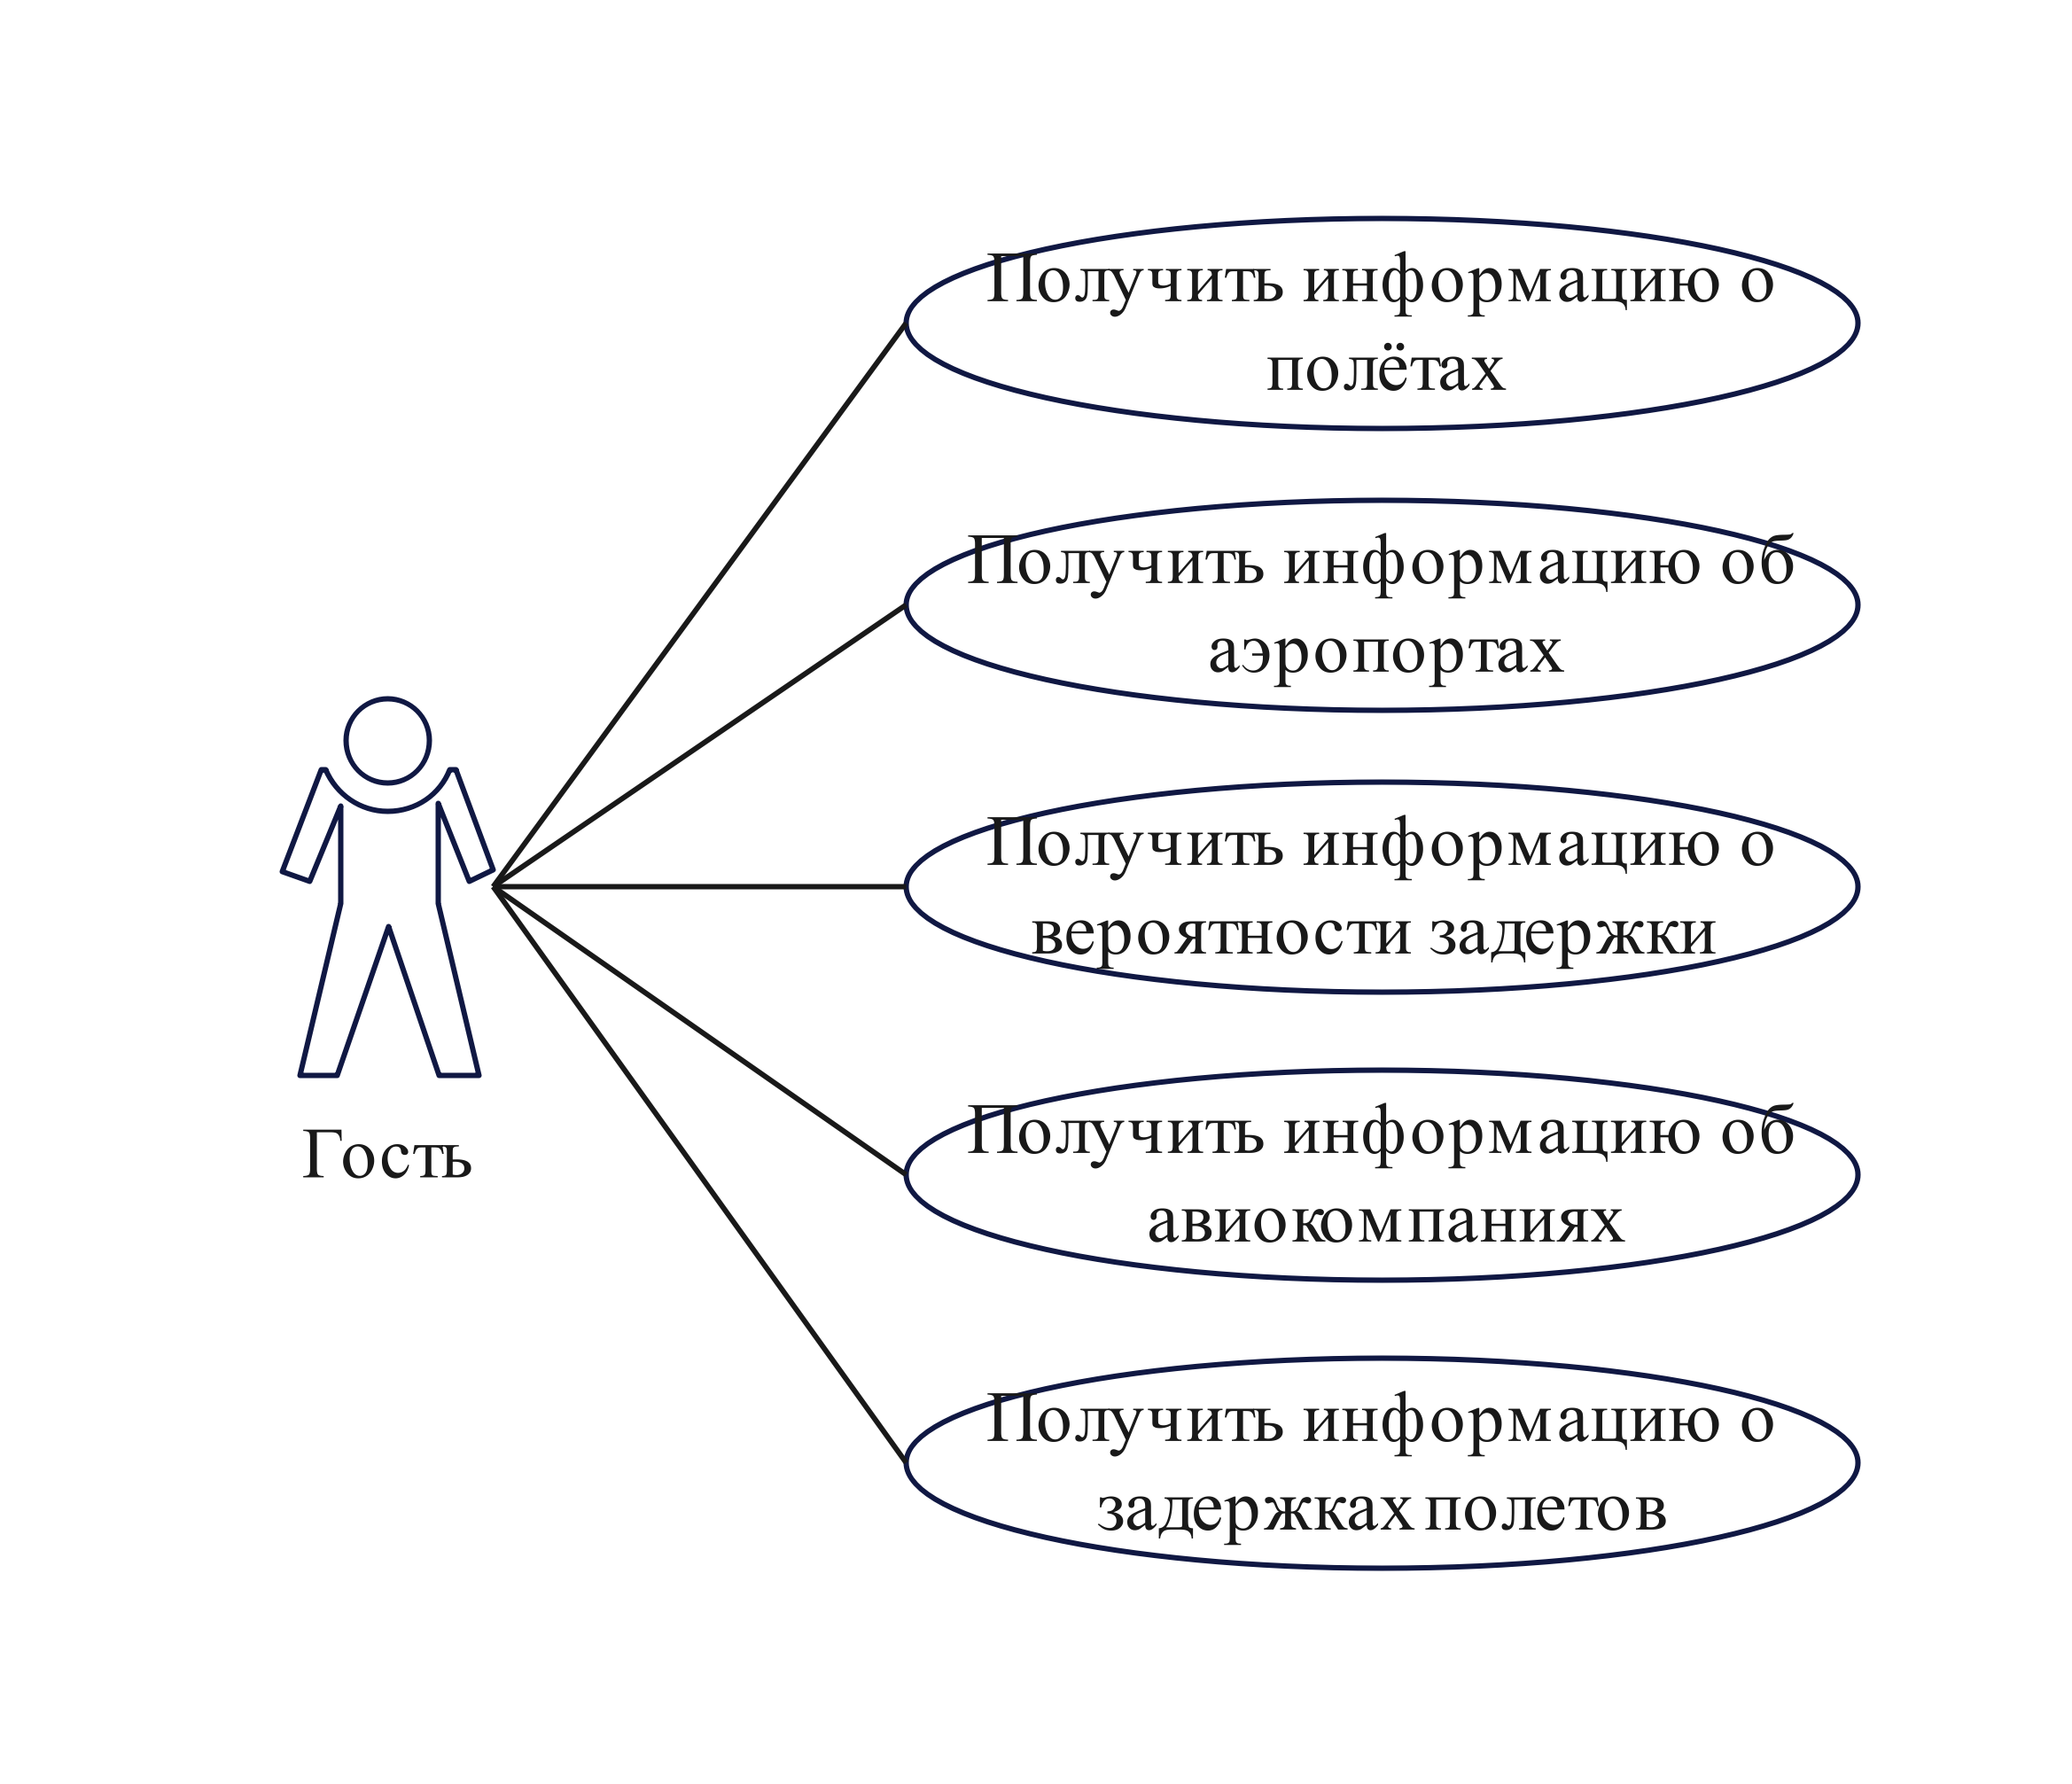
\includegraphics[scale=0.7]{inc/Guest_role}
        \caption{Use--case диаграмма для роли "гость"}
        \label{fig:guest_role}
    \end{figure}

    \item сотрудник --- пользователь, который имеет доступ к чтению и записи сущностей отчета и системы;
    \begin{figure}[H]
        \centering
        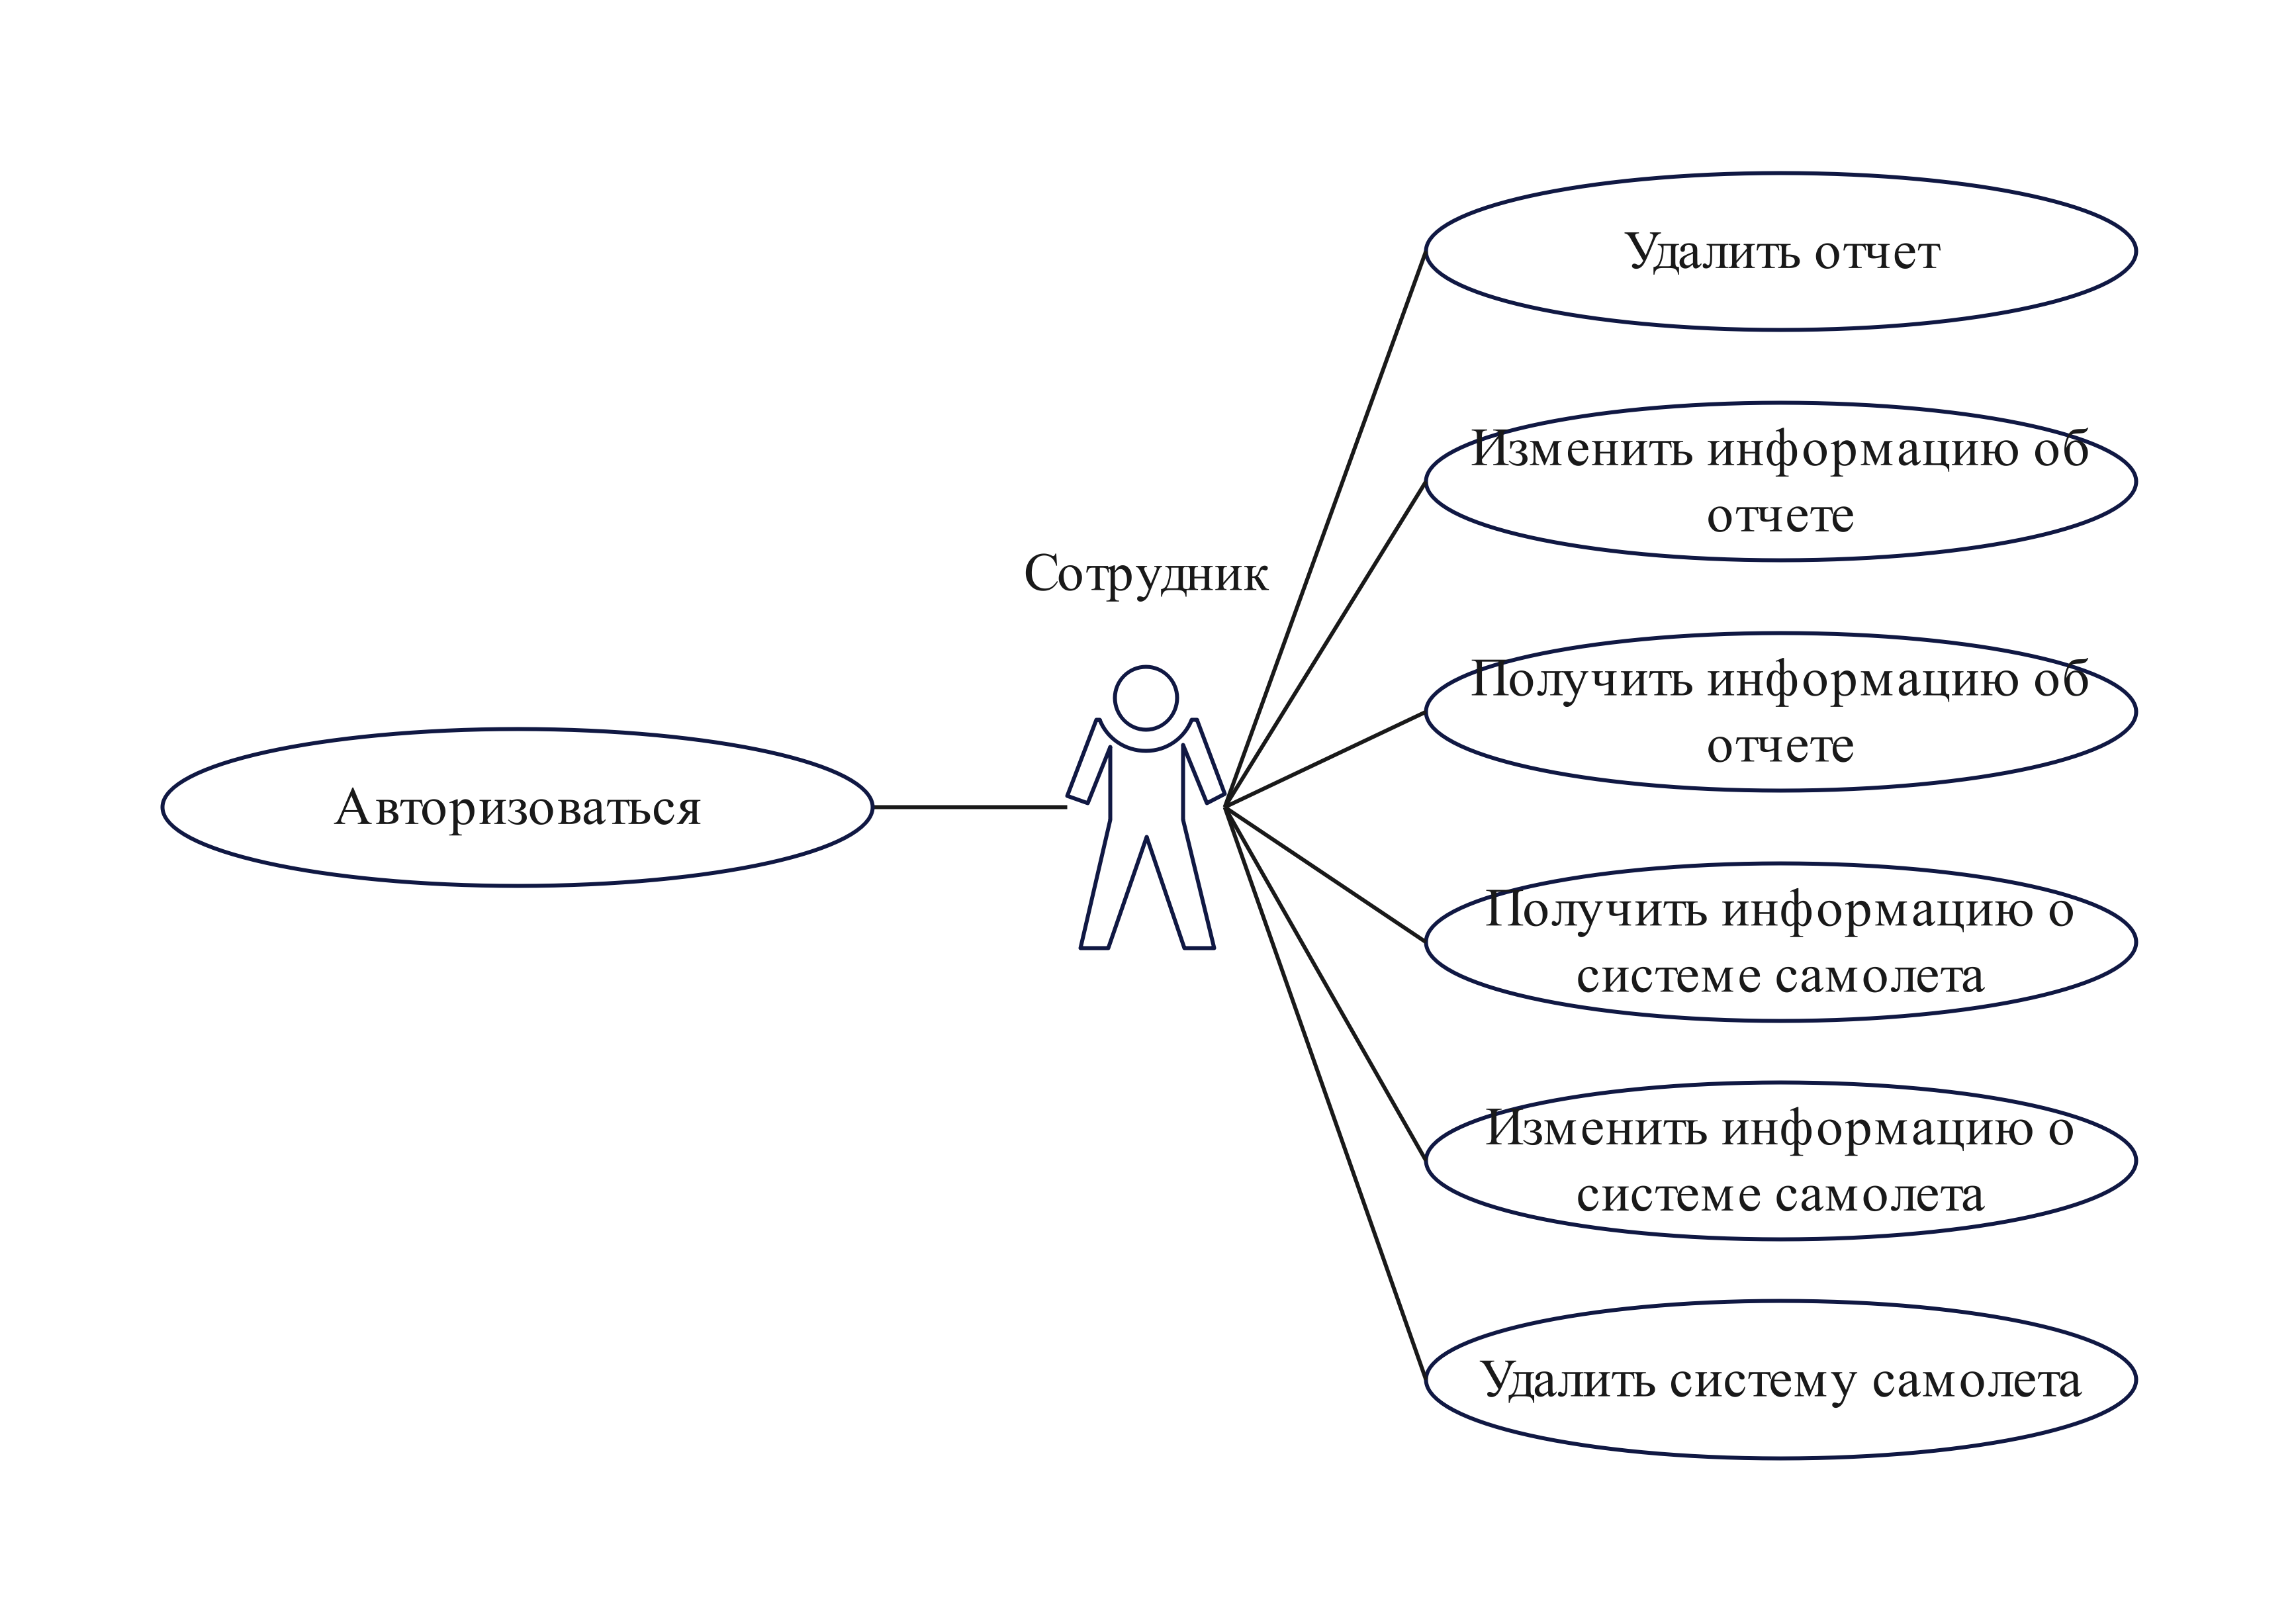
\includegraphics[scale=0.7]{inc/Employee_role}
        \caption{Use--case диаграмма для роли "сотрудник"}
        \label{fig:client_role}
    \end{figure}

    \item администратор --- пользователь, имеющий полный контроль над всеми сущностями, а также возможность получить информацию о вероятности задержки конкретного перелета.
    \begin{figure}[H]
        \centering
        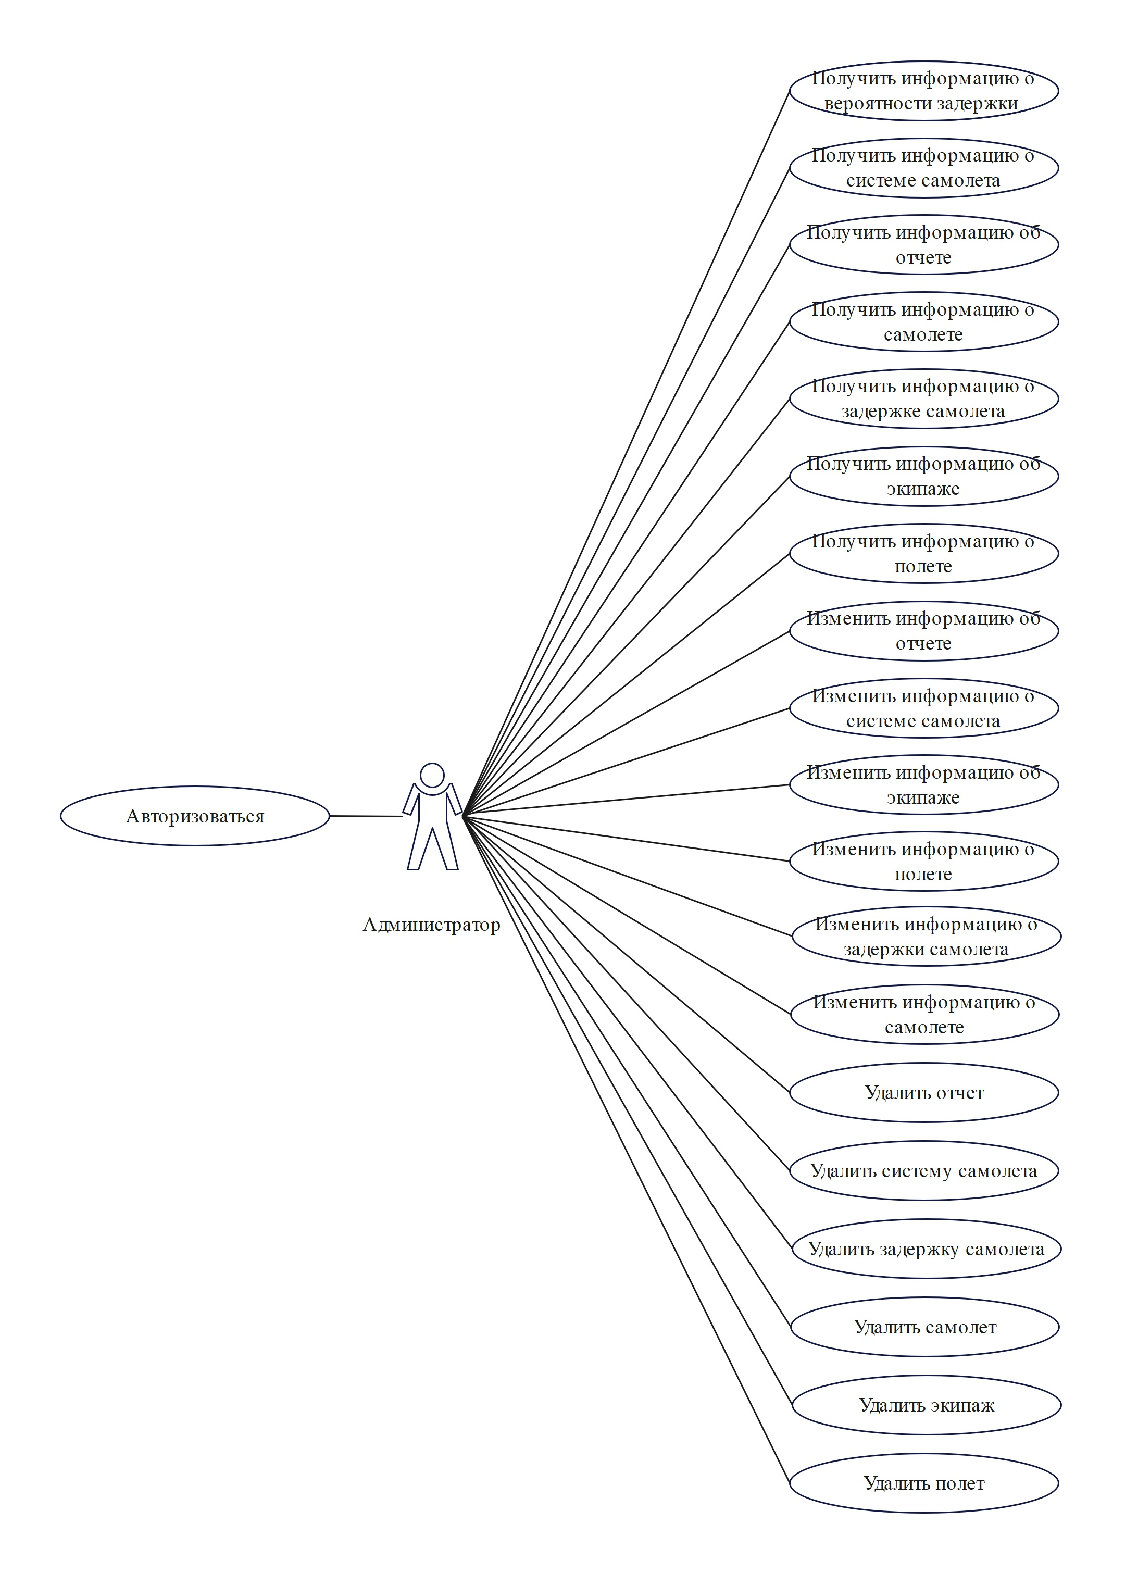
\includegraphics[scale=0.7]{inc/Admin_role}
        \caption{Use--case диаграмма для роли "администратор"}
        \label{fig:admin_role}
    \end{figure}
\end{enumerate}
\newpage


\section{Выбор модели базы данных}
По модели хранения данных выделяют следующие СУБД \newline(\textit{англ.} DBMS --- database management system):

\begin{enumerate}[label=\arabic*)]
    \item дореляционные;
    \item реляционные;
    \item постреляционные.
\end{enumerate}

Ниже рассмотрены основные модели баз данных.

\subsection{Дореляционные СУБД}
\begin{enumerate}[label=\arabic*.]
    \item Инвертированные списки --- БД на основе инвертированных списков представляет собой совокупность файлов, содержащих записи (таблиц).
    Для записей в файле определен некоторый порядок, диктуемый физической организацией данных.
    Для каждого файла может быть определено произвольное число других упорядочений на основании значений некоторых полей записей (инвертированных списков).
    Обычно для этого используются индексы.
    В такой модели данных отсутствуют ограничения целостности как таковые.
    Все ограничения на возможные экземпляры БД задаются теми программами, которые работают с БД.
    Одно из немногих ограничений, которое все-таки может присутствовать - это ограничение, задаваемое уникальным индексом~\cite{lekcii}.
    \item Иерархическая модель данных --- иерархическая модель БД состоит из объектов с указателями от родительских объектов к потомкам, соединяя вместе связанную информацию.
    Иерархические БД могут быть представлены в виде дерева~\cite{lekcii}.
    \item Сетевая модель данных --- к основным понятиям сетевой модели БД относятся: элемент (узел), связь.
    Узел — это совокупность атрибутов данных, описывающих некоторый объект.
    Сетевые БД могут быть представлены в виде графа.
    В сетевой БД логика процедуры выборки данных зависит от физической организации этих данных.
    Поэтому эта модель не является полностью независимой от приложения.
    Другими словами, если необходимо изменить структуру данных, то нужно изменить и приложение~\cite{lekcii}.

    На рисунке~\ref{fig:network-model} представлена сетевая модель данных.

    \begin{figure}[h]
        \begin{center}
            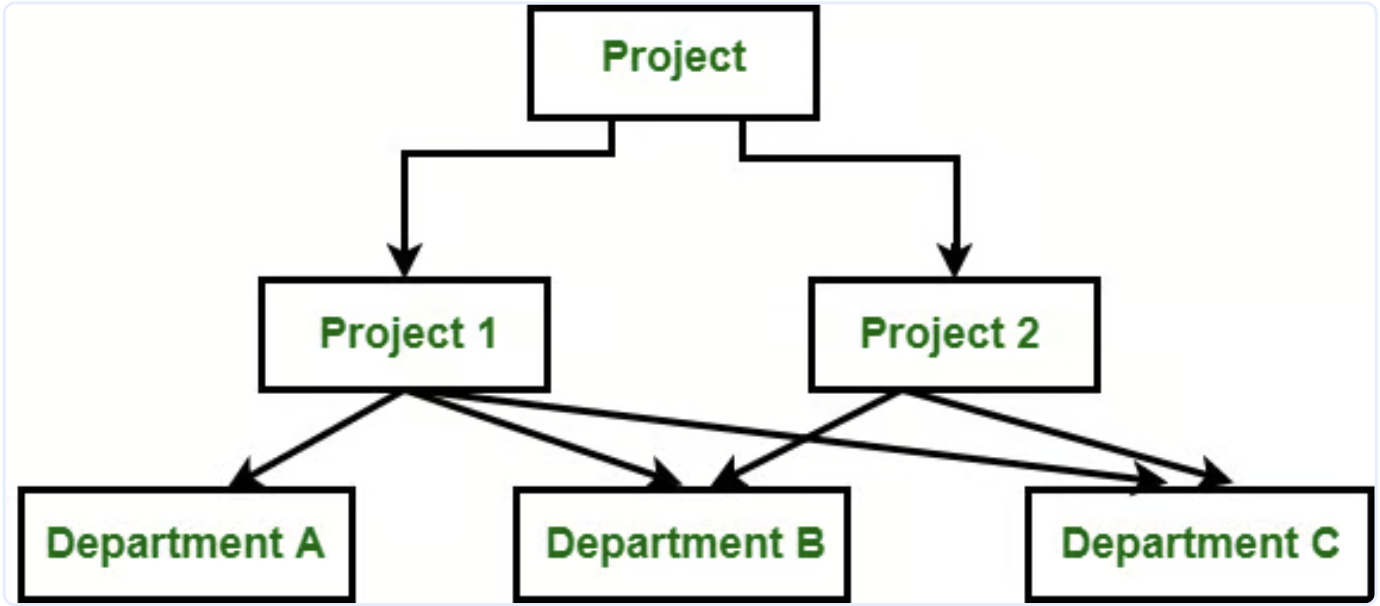
\includegraphics[scale=0.3]{inc/network-model}
            \caption{Сетевая модель данных}
            \label{fig:network-model}
        \end{center}
    \end{figure}
\end{enumerate}

\subsection{Реляционная модель данных}
Реляционная модель данных включает в себя следующие аспекты:

\begin{enumerate}[label=\arabic*)]
    \item структурный аспект --- данные в базе данных представлены в виде набора отношений, также известных как таблицы.
    \item целостностный аспект --- отношения (таблицы) должны соответствовать определенным условиям целостности, гарантирующим правильное и надежное хранение данных.
    \item манипуляционный аспект --- манипулирование данными в отношениях осуществляется с помощью средств реляционной алгебры и/или реляционного исчисления.
    Это позволяет выполнять различные операции над данными, такие как выборка, вставка, обновление и удаление.
    Кроме того, реляционная модель данных включает в себя теорию нормализации, которая помогает улучшить организацию данных в базе данных и избежать избыточности и аномалий.
    В 1985 году доктор Кодд сформулировал двенадцать правил, которым должна соответствовать настоящая реляционная база данных.
    Эти правила являются полуофициальным определением понятия реляционной базы данных и предоставляют стандарт для оценки соответствия реляционной базы данных этой модели~\cite{lekcii}.
\end{enumerate}


\section*{Выводы}
В данном разделе проанализированы техническое обслуживание самолетов, процесс оборота самолета и наземное обслуживание.
Определены требования к разрабатываемой базе данных, выделены основные сущности для хранения данных.
Разработана система ролей для пользователей на уровне базы данных.
Выбрана реляционная модель данных для реализации базы данных.


\chapter{Конструкторский раздел}

В данном разделе будут описаны проектируемая база данных, используемый триггер и хранимая процедура, а также система ролей в базе данных.

\section{Проектируемая база данных}

На рисунке~\ref{fig:uml} представлена диаграмма проектируемой базы данных.
\begin{figure}[H]
    \centering
    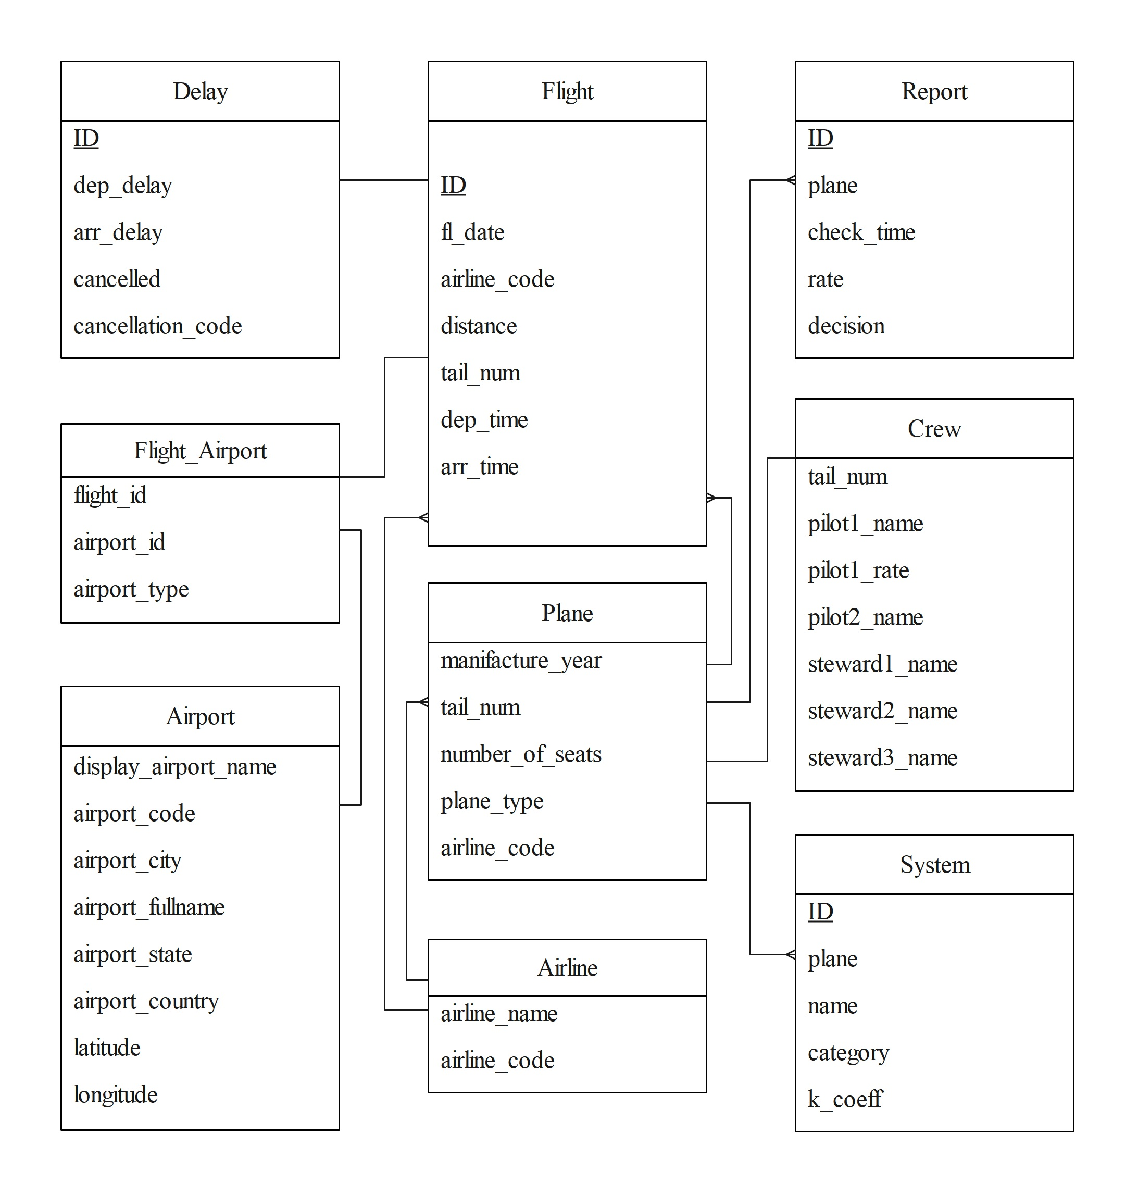
\includegraphics[scale=0.6]{inc/Drawing3}
    \caption{Диаграмма проектируемой базы данных}
    \label{fig:uml}
\end{figure}

\newpage
В таблицах~\ref{tab:tabl1}--~\ref{tab:tabl9} представлены описания полей соответствующих таблиц базы данных:

\begin{table}[H]
    \centering
    \captionsetup{justification=centering}
    \caption{Описание таблицы flight}
    \begin{tabular}{|p{0.4\textwidth}|p{0.4\textwidth}|}
        \hline
        Атрибут & Тип данных \\
        \hline
        Идентификатор & Целое число \\
        Дата вылета & Дата \\
        Код авиакомпании & Строка \\
        Время вылета & Время \\
        Время прилета & Время \\
        Номер борта & Строка \\
        \hline
    \end{tabular}
    \label{tab:tabl1}
\end{table}

\begin{table}[H]
    \centering
    \captionsetup{justification=centering}
    \caption{Описание таблицы delay}
    \begin{tabular}{|p{0.4\textwidth}|p{0.4\textwidth}|}
        \hline
        Атрибут & Тип данных \\
        \hline
        Идентификатор & Целое число \\
        Задержка вылета & Вещественное число \\
        Задержка прилета & Вещественное число \\
        Статус & Целое число \\
        Причина отмены & Строка \\
        \hline
    \end{tabular}
    \label{tab:tabl2}
\end{table}

\begin{table}[H]
    \centering
    \captionsetup{justification=centering}
    \caption{Описание таблицы airport}
    \begin{tabular}{|p{0.4\textwidth}|p{0.4\textwidth}|}
        \hline
        Атрибут & Тип данных \\
        \hline
        Название & Строка \\
        Код аэропорта & Строка \\
        Город & Строка \\
        Полное имя & Строка \\
        Страна & Строка \\
        Географская ширина & Вещественное число \\
        Географская высота & Вещественное число \\
        \hline
    \end{tabular}
    \label{tab:tabl3}
\end{table}

\begin{table}[H]
    \centering
    \captionsetup{justification=centering}
    \caption{Описание таблицы airline}
    \begin{tabular}{|p{0.4\textwidth}|p{0.4\textwidth}|}
        \hline
        Атрибут & Тип данных \\
        \hline
        Название & Строка \\
        Код авиакомпании & Строка \\
        \hline
    \end{tabular}
    \label{tab:tabl4}
\end{table}

\begin{table}[H]
    \centering
    \captionsetup{justification=centering}
    \caption{Описание таблицы plane}
    \begin{tabular}{|p{0.4\textwidth}|p{0.4\textwidth}|}
        \hline
        Атрибут & Тип данных \\
        \hline
        Год выпуска & Целое число \\
        Номер борта & Строка \\
        Количество мест & Целое число \\
        Модель & Строка \\
        Код авиакомпании & Строка \\
        \hline
    \end{tabular}
    \label{tab:tabl5}
\end{table}

\begin{table}[H]
    \centering
    \captionsetup{justification=centering}
    \caption{Описание таблицы crew}
    \begin{tabular}{|p{0.4\textwidth}|p{0.4\textwidth}|}
        \hline
        Атрибут & Тип данных \\
        \hline
        Номер борта & Строка \\
        ФИО первого пилота & Строка \\
        ФИО второго пилота & Строка \\
        ФИО первого стююарда & Строка \\
        ФИО второго стьюарда & Строка \\
        ФИО третьего стьюарда & Строка \\
        \hline
    \end{tabular}
    \label{tab:tabl6}
\end{table}

\begin{table}[H]
    \centering
    \captionsetup{justification=centering}
    \caption{Описание таблицы report}
    \begin{tabular}{|p{0.4\textwidth}|p{0.4\textwidth}|}
        \hline
        Атрибут & Тип данных \\
        \hline
        Идентификатор & Целое число \\
        Номер борта & Строка \\
        Время создания отчета & Время \\
        Оценка & Вещественное число \\
        Решение & Логический тип \\
        \hline
    \end{tabular}
    \label{tab:tabl7}
\end{table}

\begin{table}[H]
    \centering
    \captionsetup{justification=centering}
    \caption{Описание таблицы system}
    \begin{tabular}{|p{0.4\textwidth}|p{0.4\textwidth}|}
        \hline
        Атрибут & Тип данных \\
        \hline
        Идентификатор & Целое число \\
        Номер борта & Строка \\
        Имя & Строка \\
        Категория & Строка \\
        Коэффициент износа & Вещественное число \\
        \hline
    \end{tabular}
    \label{tab:tabl8}
\end{table}

\begin{table}[H]
    \centering
    \captionsetup{justification=centering}
    \caption{Описание таблицы flight\_airport}
    \begin{tabular}{|p{0.4\textwidth}|p{0.4\textwidth}|}
        \hline
        Атрибут & Тип данных \\
        \hline
        Идентификатор полета & Целое число \\
        Идентификатор аэропорта & Целое число \\
        Тип аэропорта & Строка \\
        \hline
    \end{tabular}
    \label{tab:tabl9}
\end{table}

\section{Описание используемого триггера}

Для автоматического обновления данных в таблице system при добавлении нового отчета о самолете в таблицу report был создан триггер, который автоматически обновляет поле k\_coeff всех систем таблицы system, которые относятся к самолету.

На рисунке~\ref{fig:trigger} изображена схема алгоритма функции триггера.

\begin{figure}[H]
    \centering
    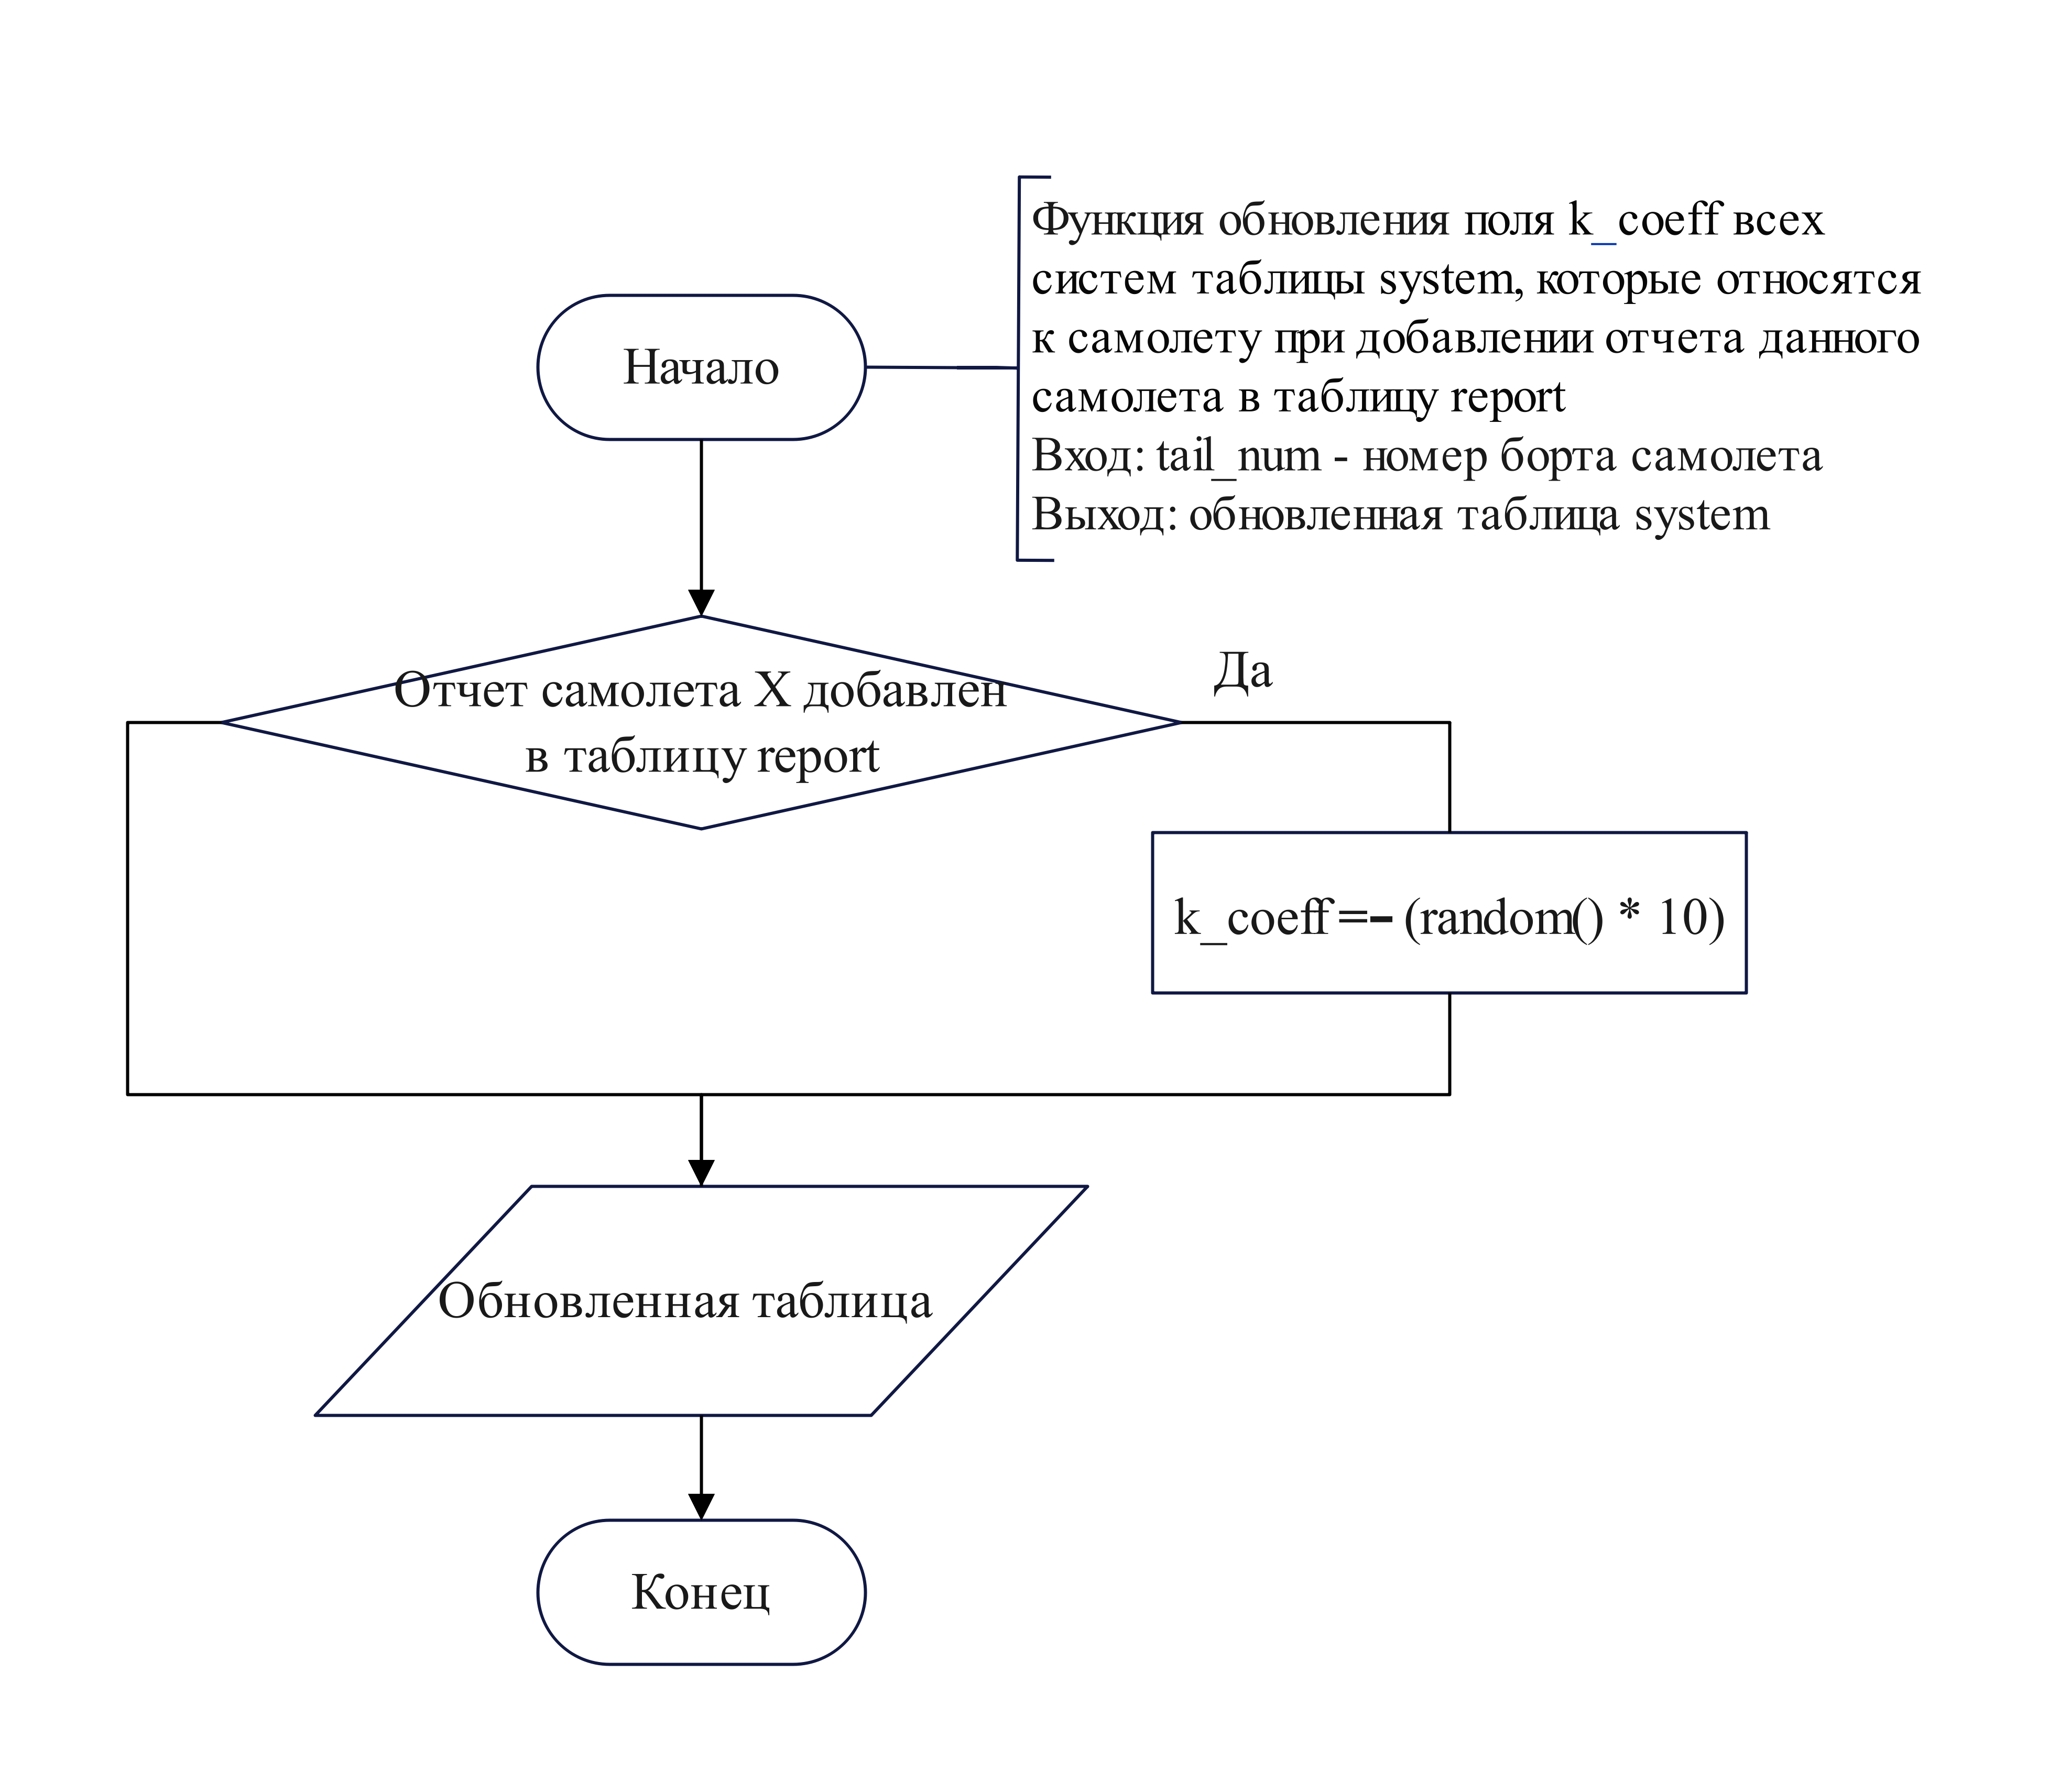
\includegraphics[scale=0.8]{inc/Drawing4}
    \caption{Схема алгоритма функции триггера}
    \label{fig:trigger}
\end{figure}

\section{Описание используемой хранимой \newline процедуры}

Для получения информации о вероятности задержки рейса была создана хранимая процедура, которая принимает на вход идентификаторы полета, аэропортов взлета и посадки, а также дату, до которой производится перебор всех полетов для вычисления вероятности задержки.

На рисунке~\ref{fig:procedure} изображена схема алгоритма хранимой процедуры.

\begin{figure}[H]
    \centering
    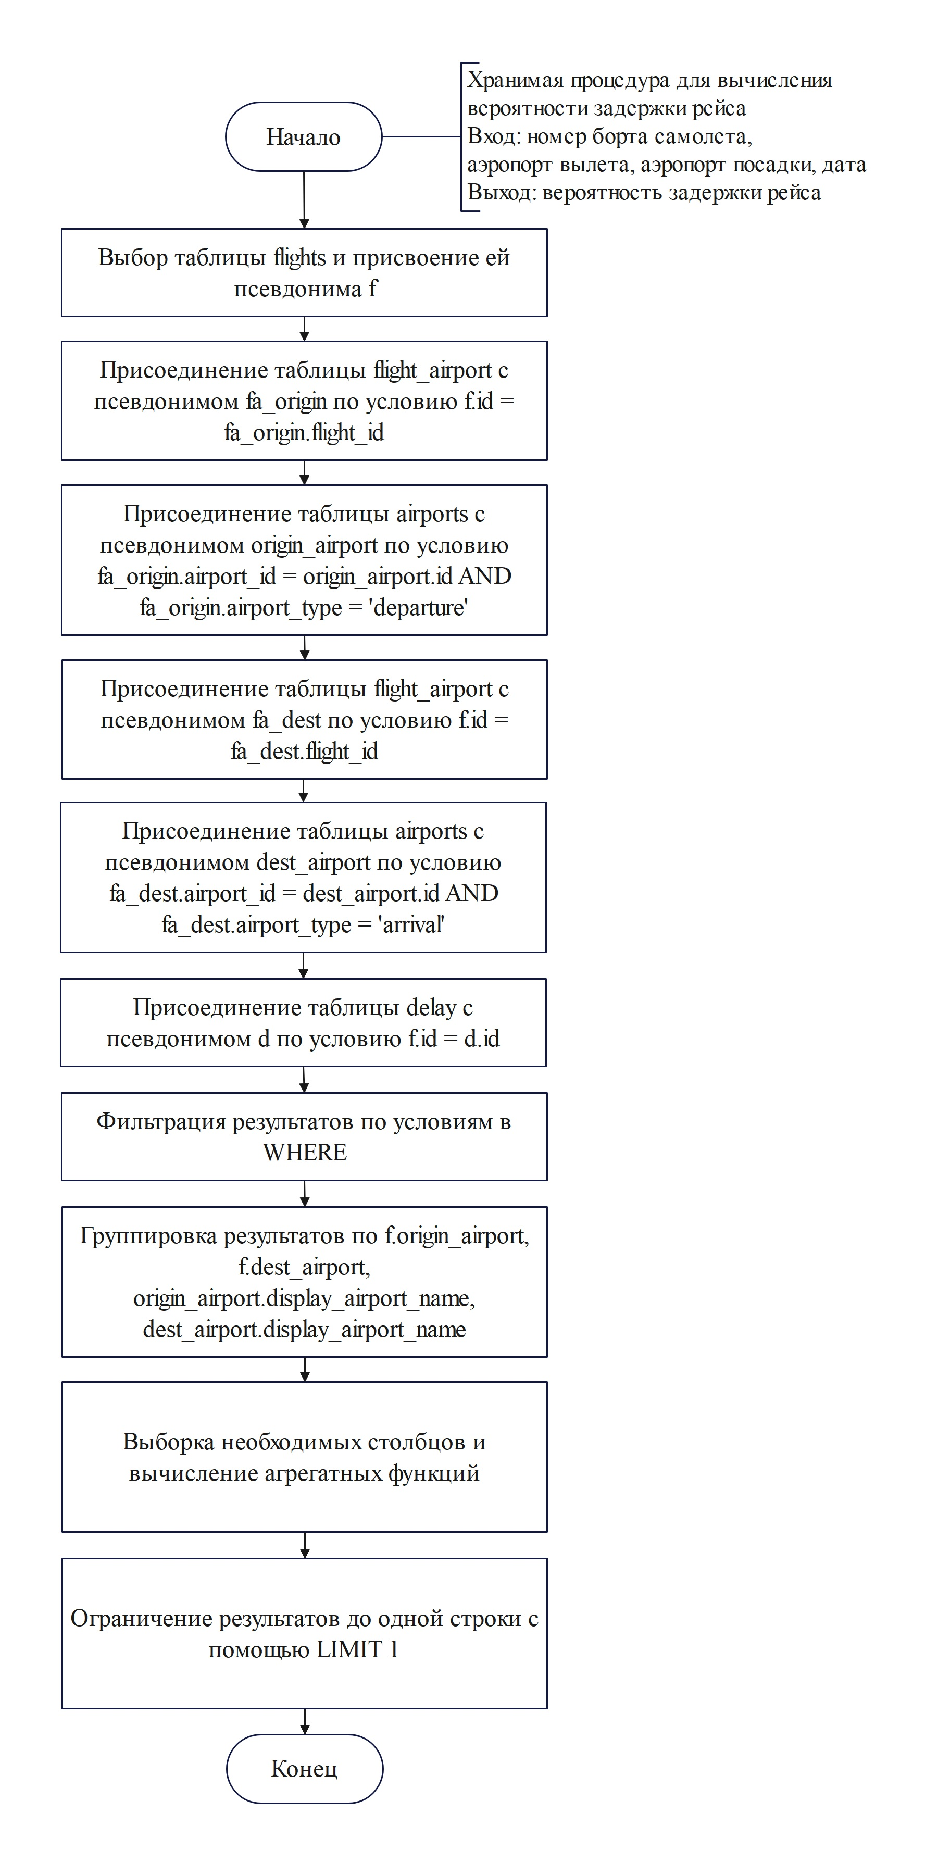
\includegraphics[scale=0.7]{inc/Drawing5}
    \caption{Схема алгоритма хранимой процедуры}
    \label{fig:procedure}
\end{figure}

Для вычисления вероятности задержки рейса была использована формула:
\begin{equation}
    P = \frac{N_{\text{задержанных}}}{N_{\text{всех}}}, \label{eq:prob}
\end{equation}
где $N_{\text{задержанных}}$ --- количество задержанных рейсов, $N_{\text{всех}}$ --- общее количество рейсов.

Вероятность задержки рассчитывается как отношение количества задержанных рейсов к общему числу рейсов для конкретного самолета, места взлета и посадки до указанной даты.

\section{Система ролей в базе данных}

В контексте разработанной базы данных были определены три основные роли: гость, сотрудник и администратор.
Эти роли были созданы для обеспечения разграничения доступа к данным и функциональности базы данных.

\begin{enumerate}[label=---]
    \item Роль ``Гость'' предоставляет возможность просмотра информации о полетах, аэропортах, авиакомпаниях и задержках, а также может получить информацию о вероятности задержки конкретного перелета.
    Это обеспечивает доступ к общедоступной информации без возможности ее изменения.
    \item Роль ``Сотрудник'' предоставляет возможность просмотра, добавления или изменения информации о системах самолетов и отчетах.
    Это позволяет сотрудникам обновлять и поддерживать актуальность данных, необходимых для их работы, при этом ограничивая их доступ только к определенным частям базы данных.
    \item Роль ``Администратор'' предоставляет полный доступ к функциональности базы данных, включая просмотр, добавление или изменение информации о полетах, аэропортах, авиакомпаниях, самолетах, задержках, экипаже, системах самолетов и отчетах.
    Администратор также может получить информацию о вероятности задержки конкретного перелета.
\end{enumerate}

Система ролей является важным элементом обеспечения безопасности и целостности данных.
Она позволяет контролировать доступ к данным и предотвращает несанкционированные изменения или удаление информации.

\chapter{Технологический раздел}

В этом разделе осуществляется выбор инструментов для реализации, предоставляется описание разрабатываемой базы данных и ее структуры, а также приводятся примеры работы программы.

\section{Технологии, используемые при \newline создании ПО}

Для выполнения данной курсовой работы был выбран язык \newline $Python$~\cite{python-lang}.

Для взаимодействия с базами данных в объектно--ориентированной парадигме была выбрана технология $SQLAlchemy$~\cite{sqlalchemy}.

Для работы с базой данных была выбрана СУБД $PostgreSQL$~\cite{postgresql}.

\section{Архитектура ПО}

В процессе разработки были реализованы следующие структуры:
\begin{enumerate}[label=\arabic*)]
    \item Flight --- описывает информацию о полете;
    \item Delay --- описывает информацию о задержке;
    \item Airport --- описывает информацию об аэропорте;
    \item Airline --- описывает информацию об авиакомпании;
    \item Plane --- описывает информацию о самолете;
    \item Crew --- описывает информацию о членах экипажа;
    \item Report --- описывает информацию о отчетах;
    \item System --- описывает информацию о системах;
\end{enumerate}

Также была создана функция, проверяющая наличие необходимой роли у пользователя для выполнения отправленного запроса.

\section{Реализация триггера}

В листинге~\ref{lst:trigger} представлен триггер для обновления данных в таблице system при добавлении нового отчета о самолете в таблицу report.

\begin{lstlisting}[label=lst:trigger, caption=Триггер для обновления данных в таблице system, language=SQL]
def create_trigger(db: Session):
    sql = """
    CREATE OR REPLACE FUNCTION decrease_k_coeff() RETURNS TRIGGER AS $$
    BEGIN
    UPDATE systems
    SET k_coeff = k_coeff - (random() * 10)
    WHERE plane = NEW.plane;
    RETURN NEW;
    END;
    $$ LANGUAGE plpgsql;

    CREATE TRIGGER decrease_k_coeff_trigger
    AFTER INSERT ON reports
    FOR EACH ROW EXECUTE FUNCTION decrease_k_coeff();
    """
    db.execute(text(sql))
\end{lstlisting}

\section{Реализация хранимой процедуры}
В листинге~\ref{lst:procedure} представлена хранимая процедура для получения вероятности задержки рейса.

\begin{lstlisting}[label=lst:procedure, caption=Хранимая процедура для получения вероятности задержки рейса, language=SQL]
CREATE OR REPLACE PROCEDURE probability(
plane VARCHAR,
origin VARCHAR,
destination VARCHAR,
date_limit VARCHAR
)
LANGUAGE plpgsql
AS $$
BEGIN
    CREATE TEMP TABLE IF NOT EXISTS temp_result (
        airport VARCHAR,
        average_delay FLOAT,
        total_delays INT,
        delay_percentage FLOAT
    ) ON COMMIT DROP;

    INSERT INTO temp_result
    SELECT
        dest_airport.display_airport_name AS airport,
        AVG(d.dep_delay) as average_delay,
        COUNT(d.dep_delay) as total_delays,
        ((CAST(COUNT(d.dep_delay) AS FLOAT) /
        (SELECT COUNT(*) FROM flights WHERE tail_num = plane AND fl_date::DATE < date_limit::DATE)) * 100.0) as delay_percentage
    FROM
        flights f
    JOIN
        flight_airport fa_origin ON f.id = fa_origin.flight_id
    JOIN
        airports origin_airport ON fa_origin.airport_id = origin_airport.id AND fa_origin.airport_type = 'departure'
    JOIN
        flight_airport fa_dest ON f.id = fa_dest.flight_id
    JOIN
        airports dest_airport ON fa_dest.airport_id = dest_airport.id AND fa_dest.airport_type = 'arrival'
    JOIN
        delay d ON f.id = d.id
    WHERE
        f.tail_num = plane AND
        origin_airport.airport_code = origin AND
        dest_airport.airport_code = destination AND
        f.fl_date::DATE < date_limit::DATE
    GROUP BY
        dest_airport.display_airport_name;
END;
$$;
\end{lstlisting}

\section{Реализация системы ролей}

В листинге~\ref{lst:roles} представлен код создания ролей в системе, в котором выдаются права на определенные таблицы в базе данных.

\begin{lstlisting}[label=lst:roles, caption=Создание ролей в системе, language=SQL]
CREATE ROLE guest;
CREATE ROLE employee;
CREATE ROLE admin;

GRANT SELECT ON flights, airports, airlines, delay TO guest;

GRANT ALL PRIVILEGES ON reports, systems, checklist TO employee;

GRANT ALL PRIVILEGES ON ALL TABLES IN SCHEMA public TO admin;
\end{lstlisting}

\newpage
\section{Тестирование триггера}
В соответствии со схемой алгоритма триггера, указанной на Рисунке~\ref{fig:trigger}, алгоритм включает проверку наличия уже существующего отчета для самолета Х в таблице reports.
Для целей тестирования, значение, на которое уменьшается коэффициент, было заменено с random() на 10.

В таблице~\ref{tab:tabl10} представлены модульные тесты для триггера базы данных.
\begin{table}[H]
    \centering
    \captionsetup{justification=raggedright}
    \caption{Модульное тестирование триггера базы данных (ч. 1)}
    \begin{tabular}{|c|p{0.3\textwidth}|p{0.3\textwidth}|p{0.2\textwidth}|}
        \hline
        № & Класс \newline эквивалентности & Запрос для теста & Результат \\
        \hline
        1 & Вставка первого \newline отчета для самолета N10156 в таблицу reports с k\_coeff = 100 & INSERT INTO reports (tail\_num, avg\_rate, decision, datetime) VALUES ('N10156', 100, `true', `2024-06-09 00:54:53'); & k\_coeff = 90 \\
        \hline
        2 & Вставка второго \newline отчета для самолета N10156 в таблицу reports с k\_coeff = 90 & INSERT INTO reports (tail\_num, avg\_rate, decision, datetime) VALUES ('N10156', 100, `true', `2024-06-09 01:54:53'); & k\_coeff = 80 \\
        \hline
        3 & Вставка третьего отчета для самолета N10156 в таблицу reports с k\_coeff = 80 & INSERT INTO reports (tail\_num, avg\_rate, decision, datetime) VALUES ('N10156', 100, `true', `2024-06-09 02:54:53'); & k\_coeff = 70 \\
        \hline
    \end{tabular}
    \label{tab:tabl10}
\end{table}


\begin{table}[H]
    \centering
    \captionsetup{justification=raggedright}
    \caption{Модульное тестирование триггера базы данных (ч. 2)}
    \begin{tabular}{|c|p{0.3\textwidth}|p{0.3\textwidth}|p{0.2\textwidth}|}
        \hline
        № & Класс \newline эквивалентности & Запрос для теста & Результат \\
        \hline
        4 & Вставка отчета для \newline самолета N10156 в таблицу reports с \newline k\_coeff = 0 & INSERT INTO reports (tail\_num, avg\_rate, decision, datetime) VALUES ('N10156', 100, `true', `2024-06-09 02:54:53'); & k\_coeff = 0 \\
        \hline
        5 & Вставка отчета для несуществующего самолета в таблицу reports & INSERT INTO reports (tail\_num, avg\_rate, decision, datetime) VALUES ('N10157', 100, `true', `2024-06-09 02:54:53'); & Ошибка: данный самолет не существует \\
        \hline
        6 & Вставка отчета для \newline существующего \newline самолета в таблицу reports с \newline некорректными \newline данными & INSERT INTO reports (tail\_num, avg\_rate, decision, datetime) VALUES ('N10156', 100, `true', `2024-06-09 02:54:53'); & Ошибка: некорректные данные \\
        \hline
    \end{tabular}
    \label{tab:tabl11}
\end{table}

В процессе тестирования были выполнены запросы, указанные в Таблицах~\ref{tab:tabl10}-\ref{tab:tabl11}.
После их выполнения, в случае успешного завершения, проводилась проверка соответствия текущего состояния кортежа ожидаемому, и получалось сообщение, соответствующее таблице.
Если ожидался неудачный исход, проверялось наличие сообщения об ошибке, соответствующего таблице, и состояние кортежа должно было соответствовать его предыдущему состоянию.

\newpage
\section{Примеры работы}
На рисунках~\ref{fig:example_employee},~\ref{fig:example_flight},~\ref{fig:example_probability} представлены примеры работы приложения.

\begin{itemize}
    \item авторизация сотрудника;
    \begin{figure}[H]
        \centering
        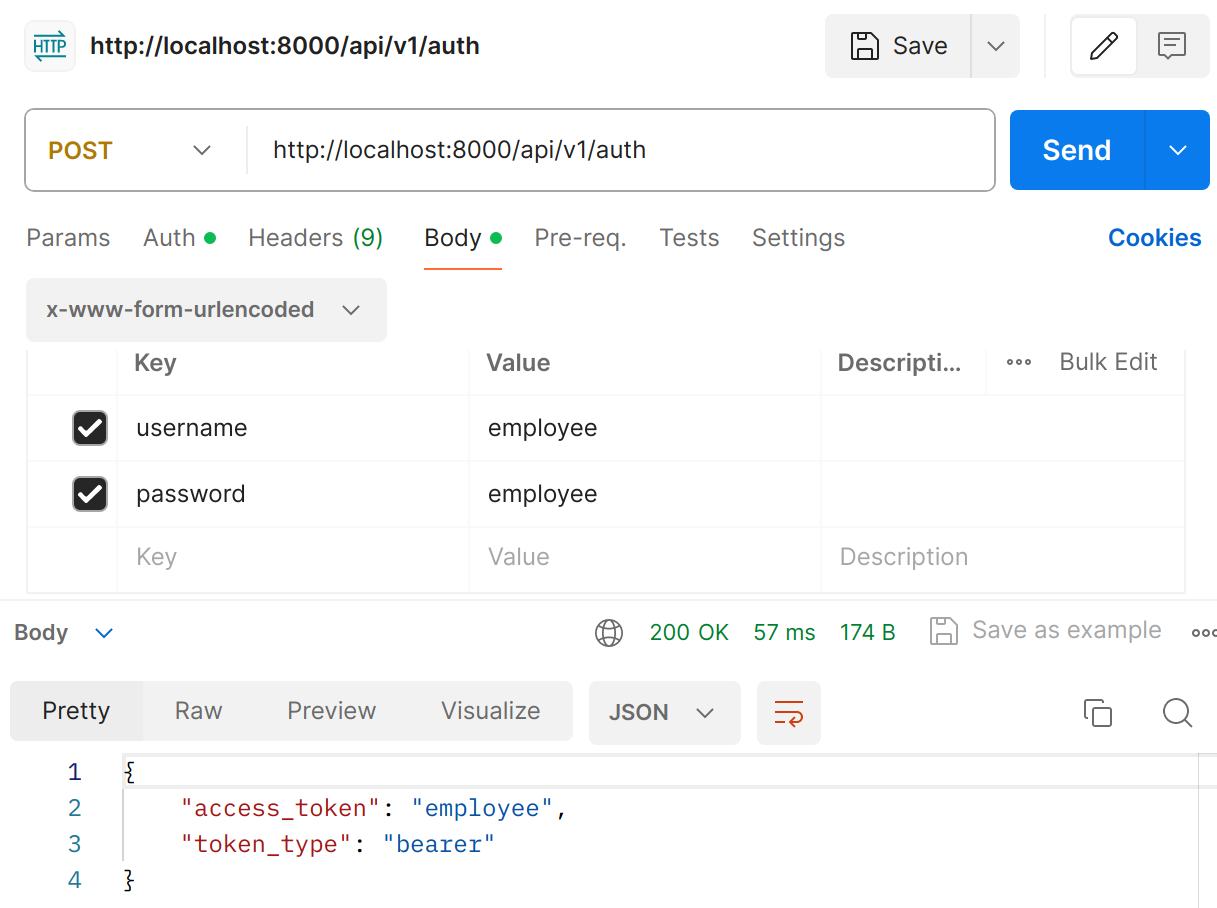
\includegraphics[scale=0.2]{inc/example_employee}
        \caption{Пример работы программы}
        \label{fig:example_employee}
    \end{figure}

    \item получение информации о полете;
    \begin{figure}[H]
        \centering
        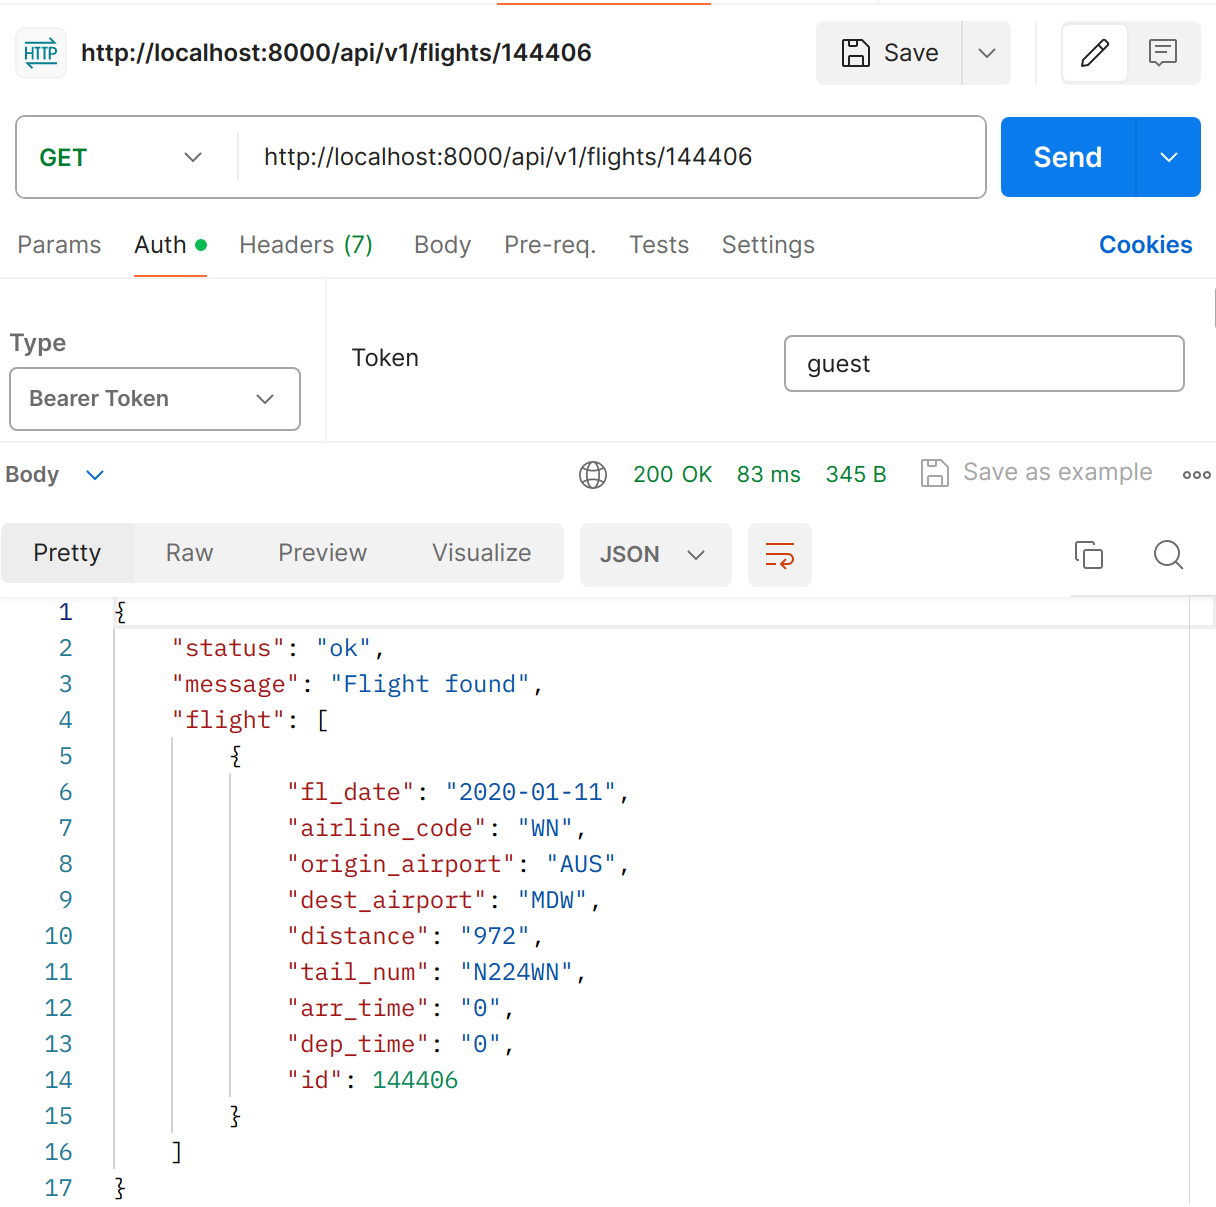
\includegraphics[scale=0.2]{inc/example_flight}
        \caption{Пример работы программы}
        \label{fig:example_flight}
    \end{figure}

    \item получение информации о вероятности задержки полета;
    \begin{figure}[H]
        \centering
        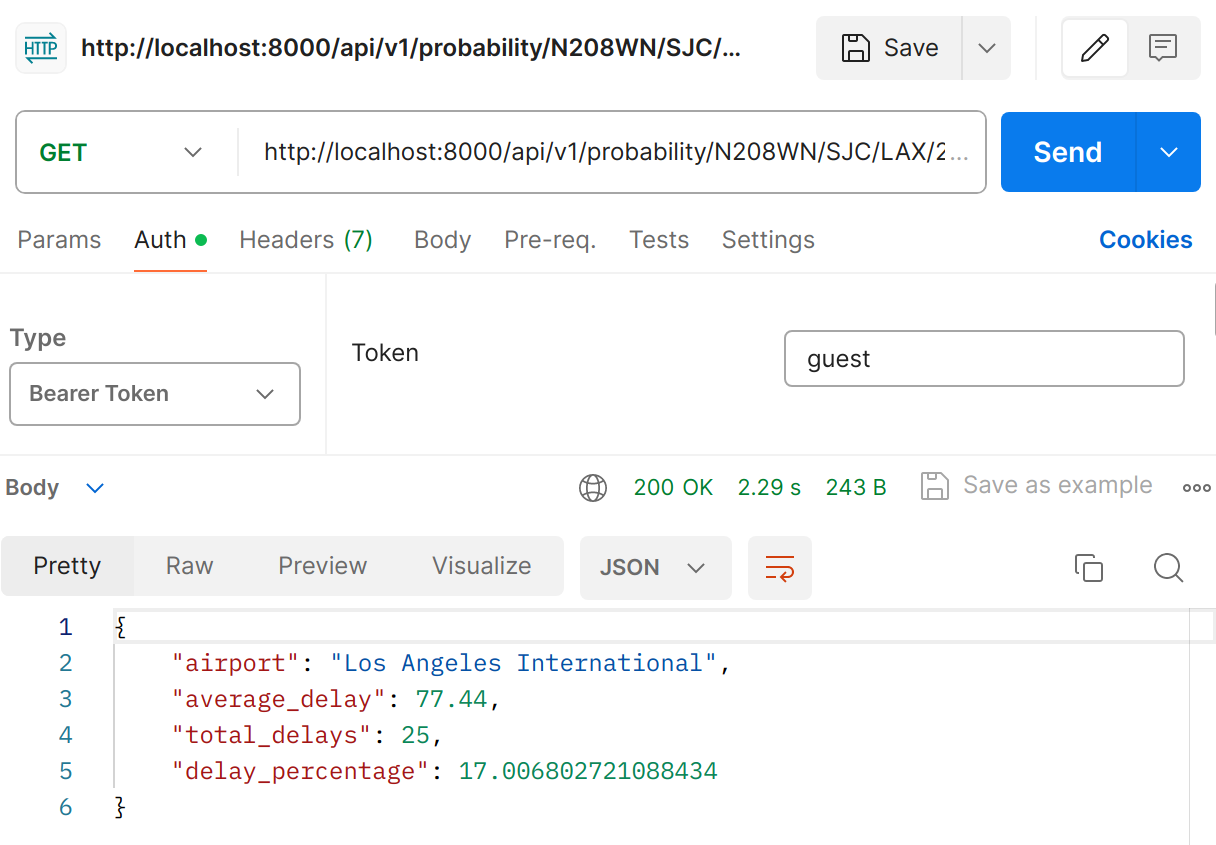
\includegraphics[scale=0.2]{inc/example_probability}
        \caption{Пример работы программы}
        \label{fig:example_probability}
    \end{figure}
\end{itemize}


\chapter{Исследовательская часть}

В данном разделе будет проведен анализ зависимости количества строк на время выполнения хранимой процедуры в базе данных.

\section{Технические характеристики}

Технические характеристики устройства, использовавшегося для выполнения замеров, представлены ниже.

\begin{itemize}[label=---]
    \item Процессор: AMD Ryzen 7--5800H with Radeon Graphics~\cite{amd_ryzen}.
    \item Оперативная память: 16 ГБайт.
    \item Операционная система: Windows 11 Home~\cite{windows}.
\end{itemize}

При замерах времени ноутбук был включен в сеть электропитания и был нагружен только системными приложениями.

\section{Сравнительный анализ работы со \newline строками в хранимой процедуре}

Время выполнения процедуры представляет собой критический параметр, определяющий производительность базы данных.
Более длительное время выполнения может привести к замедлению работы приложения и негативному влиянию на пользовательский опыт~\cite{microsoft}.

В процессе написания курсового проекта была найдена связь между количеством строк, обрабатываемых хранимой процедурой, и временем ее выполнения при работе со строками.
Для потверждения этой гипотезы был проведен сравнительный анализ работы с разным количеством строк.
В качестве хранимой процедуры была выбрана процедура, возвращающая вероятность задержки рейса.


Замеры производились на следующих параметрах:
\begin{enumerate}
    \item количество строк, обрабатываемых хранимой процедурой;
    \item время выполнения --- рассчитывается как среднее значение из 10 измерений.
\end{enumerate}

На рисунке~\ref{fig:myplot} представлен график зависимости времени выполнения хранимой процедуры от количества строк.

\begin{figure}[H]
    \centering
    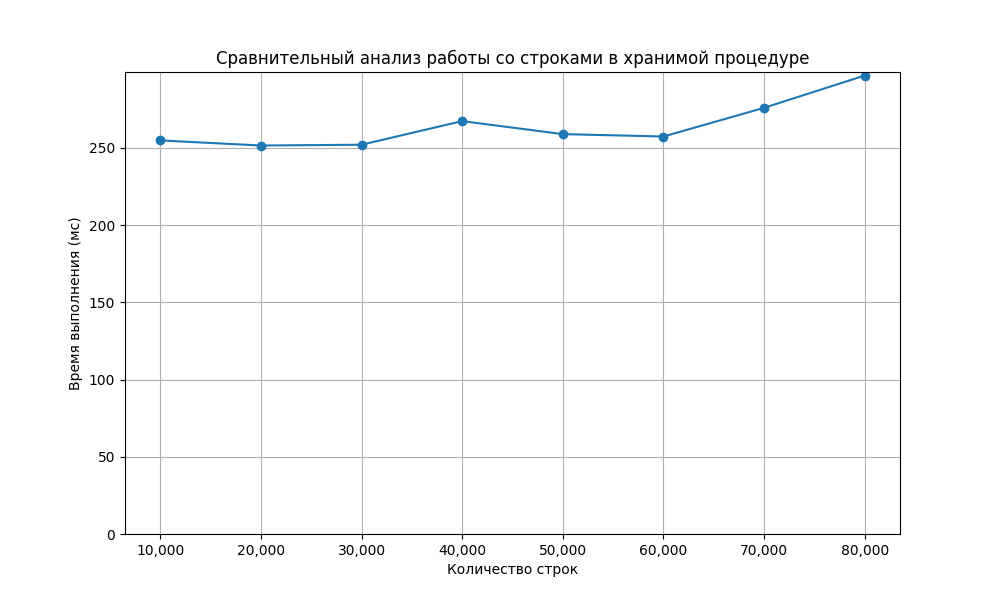
\includegraphics[scale=0.4]{inc/myplot}
    \caption{График сравнительного анализа работы со строками в хранимой процедуре}
    \label{fig:myplot}
\end{figure}

\section*{Выводы}
\addcontentsline{toc}{section}{Выводы}
В данном разделе был проведен сравнительный анализ работы с разным количеством строк в хранимой процедуре.
По результатам анализа было установлено, что время выполнения хранимой процедуры зависит от количества обрабатываемых строк --- с увеличением количества строк время выполнения хранимой процедуры линейно увеличивается.
Результаты анализа позволяют сделать выводы о том, что для оптимизации работы с базой данных необходимо уменьшать количество строк, обрабатываемых хранимой процедурой.



\addcontentsline{toc}{chapter}{ЗАКЛЮЧЕНИЕ}
\chapter*{\makebox[1.0\linewidth]{ЗАКЛЮЧЕНИЕ}}

Курсовой проект включал в себя анализ, проектирование и разработку
базы данных для прогнозирования вероятности задержки рейса в городе--пересадки из--за технического обслуживания.

На базе результатов анализа былы разработаны база данных, хранимая процедура и триггер для работы с базой данных.

Сравнительный анализ в области работы с строками в хранимой процедуре был проведен на основе замеров времени выполнения.
Было установлено, что время выполнения хранимой процедуры зависит от количества обрабатываемых строк --- с увеличением количества строк время выполнения хранимой процедуры линейно увеличивается.
Результаты анализа позволяют сделать выводы о том, что для оптимизации работы с базой данных необходимо уменьшать количество строк, обрабатываемых хранимой процедурой
и использовать другие методы для работы с данными.

Цель курсовой работы была достигнута.
В ходе выполнения работы были выполнены следующие задачи:
\begin{enumerate}[label=\arabic*)]
    \item проведен анализ предметной области;
    \item спроектирована и разработана база данных в соответствии с поставленной задачей;
    \item выбраны средства реализации базы данных и приложения;
    \item проведен сравнительный анализ работы со строками в хранимой процедуре.
\end{enumerate}


\chapter{Анализ предметной области}

\section{Регрессия}

\textbf{Определение:} Регрессия — это метод прогнозирования и анализа зависимости целевой переменной от одной или нескольких независимых переменных.
Этот подход широко применяется в задачах предсказания, моделирования и объяснения зависимости переменных, позволяя строить аналитические модели, описывающие взаимодействия в сложных системах~\cite{seber, montgomery}.

Модель регрессии предсказывает числовое значение.
Например, модель погоды, которая прогнозирует количество дождя в миллиметрах, является регрессионной моделью.

В таблице~\ref{tab:tabl1} приведены примеры регрессионных моделей.

\begin{table}[ht]
    \centering
    \caption{Примеры регрессионных моделей}
    \begin{tabularx}{\textwidth}{|>{\centering\arraybackslash}X|>{\centering\arraybackslash}X|>{\centering\arraybackslash}X|}
        \hline
        Сценарий & Входные данные & Выходные данные \newline(числовой прогноз) \\
        \hline
        Будущая цена дома & Площадь участка, количество спален и ванных комнат, размер участка, процентная ставка по ипотеке, ставка налога на недвижимость, затраты на строительство и количество домов, выставленных на продажу в этом районе & Цена дома \\
        \hline
        Будущее время поездки & Исторические условия дорожного движения, расстояние до пункта назначения и погодные условия & Время в минутах и секундах до прибытия в пункт назначения \\
        \hline
    \end{tabularx}
    \label{tab:tabl1}
\end{table}

Существует множество видов регрессии, и в данной работе будут рассмотрены следующие три вида регрессии: линейная регрессия, логистическая регрессия и адаптивная регрессия.

\chapter{Обзор существующих решений задачи регрессии}
\section{Линейная регрессия}

\textbf{ Определение:} Линейная регрессия --- это статистический метод, используемый для поиска взаимосвязи между переменными.
В контексте машинного обучения линейная регрессия находит связь между функциями и меткой~\cite{google}.

Линейная регрессия является одним из наиболее популярных алгоритмов и чаще всего используется для начала решения любой задачи регрессии, так как считается простейшей моделью машинного обучения~\cite{kemer}.

В математической статистике линейная регрессия представляет собой метод аппроксимации зависимостей между входными и выходными переменными на основе линейной модели~\cite{loginom}.

Если рассматривается зависимость между одной входной и одной выходной переменными, то имеет место простая линейная регрессия.
Уравнение регрессии для этого случая имеет вид:
\begin{equation}
    y = ax + b,
\end{equation}
где $a$ --- коэффициент наклона (или угловой коэффициент) линии регрессии, $b$ --- свободный член (перехват с осью $y$).

Коэффициенты $a$ и $b$, называемые также параметрами модели, определяются таким образом, чтобы сумма квадратов отклонений точек, соответствующих реальным наблюдениям данных, от линии регрессии была бы минимальной~\cite{loginom}.
Коэффициенты обычно оцениваются методом наименьших квадратов по следующей формуле:
\begin{equation}
    S(a, b) = \sum_{i=1}^{n}(y_i - (ax_i + b))^2,
\end{equation}
где $y_i$ --- наблюдаемое значение зависимой переменной для i-го наблюдения, $x_i$ --- значение независимой переменной для i-го наблюдения, $ax_i + b$ --- предсказанное значение зависимой переменной.

Чтобы найти коэффициенты $a$ и $b$, минимизируем эту сумму по отношению к $a$ и $b$.
Обычно, для этого используются аналитические формулы, полученные путем дифференцирования суммы квадратов остатков:
\begin{equation}
    a = \frac{n \sum_{i=1}^{n} x_i y_i - \sum_{i=1}^{n} x_i \sum_{i=1}^{n} y_i}{n \sum_{i=1}^{n} x_i^2 - (\sum_{i=1}^{n} x_i)^2},
\end{equation}
\begin{equation}
    b = \frac{1}{n}\sum_{i=1}^{n} y_i - a\frac{1}{n}\sum_{i=1}^{n} x_i,
\end{equation}
где $n$ --- количество наблюдений.

Для оценки качества модели линейной регрессии часто используется коэффициент детерминации $R^2$, который показывает долю изменчивости зависимой переменной, объясненную моделью.
Он рассчитывается как квадрат коэффициента корреляции $r_{xy}$:
\begin{equation}
    R^2 = r_{xy}^2,
\end{equation}
где $r_{xy}$ --- коэффициент корреляции между $x$ и $y$.
Чем ближе $R^2$ к 1, тем лучше модель объясняет зависимость между переменными.

На рисунке~\ref{img:linear-regression} представлен пример построения линии регрессии.
\includeimage
{linear-regression}
{f}
{H}
{\textwidth}
{Пример построения линии регрессии}

Если рассматривается зависимость между несколькими входными и одной выходной переменными, то имеет место множественная линейная регрессия.
Соответствующее уравнение имеет вид (\ref{eq:1}):
\begin{equation}
    y = b_0 + b_1 x_1 + b_2 x_2 + \cdots+ b_n x_n,
    \label{eq:1}
\end{equation}
где $n$ --- число входных переменных.

В данном случае модель будет описываться не прямой, а гиперплоскостью.
Коэффициенты уравнения множественной линейной регрессии подбираются так, чтобы минимизировать сумму квадратов отклонения реальных точек от этой гиперплоскости~\cite{loginom}.

\subsection*{Применение}

Линейная регрессия имеет много практических применений, которые можно разделить на две основные категории:
\begin{enumerate}[label=\arabic*), leftmargin=1.6\parindent]
    \item прогнозирование --- линейную регрессию можно использовать для подгонки модели к наблюдаемому набору данных;
    \item объяснение изменчивости --- линейный регрессионный анализ применяется для количественной оценки силы взаимосвязи между выходной и входными переменными.
\end{enumerate}

Оценим практическое применение способа построения линейной регрессии в экономике на примере формирования заработной платы, зависящей от показателя среднедушевого прожиточного минимума на человека, на основе представленных способов и формул.
В таблице~\ref{tab:tabl3} представлены данные, на базе которых нужно выявить зависимость показателя заработной платы от фактора $x$ по регионам России за 2016 год:

\begin{table}[H]
    \centering
    \caption{Показатели среднемесячной заработной платы под влиянием
    прожиточного минимума по регионам РФ за 2016 г., тыс. руб.}
    \begin{tabularx}{\textwidth}{|>{\centering\arraybackslash}X|>{\centering\arraybackslash}X|>{\centering\arraybackslash}X|}
        \hline
        № & Среднедушевой прожиточный min на одного работающего (х) & Среднемесячная заработная плата (у) \\
        \hline
        1 & 8.70 & 17.8 \\
        \hline
        2 & 6.30 & 11.6 \\
        \hline
        3 & 7.89 & 15.8 \\
        \hline
        4 & 10.24 & 13.5 \\
        \hline
        5 & 10.25 & 20.5 \\
        \hline
        6 & 7.50 & 15.9 \\
        \hline
        7 & 8.75 & 14.9 \\
        \hline
        8 & 6.20 & 10.3 \\
        \hline
        9 & 9.86 & 18.6 \\
        \hline
        10 & 8.50 & 14.2 \\
        \hline
    \end{tabularx}
    \label{tab:tabl3}
\end{table}

С помощью представленных данных построим линейное уравнений простой регрессии.
Для этого необходимо просчитать коэффициенты $a$ и $b$.
Для упрощения расчетов построим вспомогательную таблицу~\ref{tab:tabl4}:

\begin{table}[H]
    \centering
    \caption{Расчетная таблица параметров линейного уравнения регрессии}
    \begin{tabularx}{\textwidth}{|>{\centering\arraybackslash}X|>{\centering\arraybackslash}X|>{\centering\arraybackslash}X|>{\centering\arraybackslash}X|>{\centering\arraybackslash}X|>{\centering\arraybackslash}X|>{\centering\arraybackslash}X|>{\centering\arraybackslash}X|>{\centering\arraybackslash}X|>{\centering\arraybackslash}X|}
        \hline
        № & $x$ & $y$ & $xy$ & $x^2$ & $y^2$ & $\hat{y}$ & $y-\hat{y}$ & $(y-\hat{y})^2$ & A (\%) \\
        \hline
        1 & 8.70 & 17.8 & 154.86 & 75.69 & 316.84 & 15.74 & 2.06 & 4.26 & 12\% \\
        \hline
        2 & 6.30 & 11.6 & 73.08 & 39.69 & 134.56 & 12.09 & -0.49 & 0.24 & 4\% \\
        \hline
        3 & 7.89 & 15.8 & 124.66 & 62.25 & 249.64 & 14.51 & 1.29 & 1.67 & 8\% \\
        \hline
        4 & 10.24 & 13.5 & 138.24 & 104.8 & 182.25 & 18.08 & -4.58 & 20.95 & 34\% \\
        \hline
        5 & 10.25 & 20.5 & 210.13 & 105 & 420.25 & 18.09 & 2.41 & 5.80 & 12\% \\
        \hline
        6 & 7.50 & 15.9 & 119.25 & 56.25 & 252.81 & 13.91 & 1.99 & 3.95 & 12\% \\
        \hline
        7 & 8.75 & 14.9 & 130.38 & 76.56 & 222.01 & 15.81 & -0.91 & 0.83 & 6\% \\
        \hline
        8 & 6.20 & 10.3 & 63.86 & 38.44 & 106.09 & 11.94 & -1.64 & 2.68 & 16\% \\
        \hline
        9 & 9.86 & 18.6 & 183.4 & 97.22 & 345.96 & 17.50 & 1.10 & 1.21 & 6\% \\
        \hline
        10 & 8.50 & 14.2 & 120.7 & 72.25 & 201.64 & 15.43 & -1.23 & 1.52 & 9\% \\
        \hline
        Сумма & 84.19 & 153.1 & 1318.55 & 728.27 & 2432.05 & 153.10 & 0.00 & 43.11 & 119\% \\
        \hline
        ср.знач. & 8.419 & 15.31 & 131.855 & 72.83 & 243.21 & 15.31 & 0.00 & 4.31 & 22\% \\
        \hline
    \end{tabularx}
    \label{tab:tabl4}
\end{table}

Для расчета коэффициентов $a$ и $b$ воспользуемся формулами:
\begin{itemize}
    \item $b$ (коэффициент наклона), вычисляется по формуле:
    \begin{equation}
        b = \frac{\sum (x_i - \overline{x})(y_i - \overline{y})}{\sum (x_i - \overline{x})},
    \end{equation}
    \item $a$ (свободный член), вычисляется через средние значения по формуле:
    \begin{equation}
        a = \overline{y} - b \cdot \overline{x},
    \end{equation}
\end{itemize}

Подставим значения в формулы:
\begin{equation}
    \overline{x} = \frac{\sum x}{n} = \frac{84.19}{10} = 8.42,
\end{equation}
\begin{equation}
    \overline{y} = \frac{\sum y}{n} = \frac{153.1}{10} = 15.31,
\end{equation}
\begin{equation}
    b = \frac{1318.55}{728.27} = 1.81,
\end{equation}
\begin{equation}
    a = 15.31 - 1.51 \cdot 8.42 = 2.52.
\end{equation}

Таким образом, уравнение регрессии имеет вид:
\begin{equation}
    y = 2.52 + 1.81x.
\end{equation}

Вычисляем для уравнения коэффициент детерминации:
\begin{equation}
    R^2 = \frac{(\sum(x_i - \overline{x})(y_i - \overline{y}))^2}{\sum (x_i - \overline{x})^2(y_i - \overline{y})^2} = \frac{1318.55^2}{728.27 \cdot 2432.05} = 0.51.
\end{equation}
Это означает, что 51\% изменчивости зарплаты можно объяснить изменчивостью прожиточного минимума.
Остальные 49\% объясняются другими факторами~\cite{plehanov}.

\section{Логистическая регрессия}

\textbf{ Определение:} Логистическая регрессия --- это статистическая модель, используемая для предсказания вероятности возникновения некоторого события путем подгонки данных к логистической кривой~\cite{kras}.

Логистическая регрессия применяется для предсказания вероятности возникновения некоторого события по значениям множества признаков.
Для этого вводится так называемая зависимая переменная $y$, принимающая лишь одно из двух значений, как правило, это числа: 0 (событие не произошло), и 1 (событие произошло), и множество независимых переменных (также называемых признаками, предикторами или регрессорами) --- вещественных $x_1, x_2, \cdots, x_n$, на основе значений которых требуется вычислить вероятность принятия того или иного значения зависимой переменной~\cite{kras}.

Стандартная логистическая функция, также известная как сигмовидная функция (\textit{сигмовидная} означает «s--образная»), имеет формулу (\ref{eq:2}):
\begin{equation}
    f(x) = \frac{1}{1 + e^{-x}}.
    \label{eq:2}
\end{equation}

На рисунке~\ref{img:sigmoid_function_with_axes} показан соответствующий график сигмовидной функции.
По мере увеличения входного значения $x$ выходной сигнал сигмовидной функции приближается, но никогда не достигает 1.
Точно так же, когда входные данные уменьшаются, выходные данные сигмовидной функции приближаются, но никогда не достигают 0.
\includeimage
{sigmoid_function_with_axes}
{f}
{H}
{\textwidth}
{График сигмовидной функции}

Линейный компонент модели логистической регрессии описывается следующим уравнением (\ref{eq:3}):
\begin{equation}
    z = b_0 + b_1 x_1 + b_2 x_2 +\cdots + b_n x_n,
    \label{eq:3}
\end{equation}
где $n$ --- число входных переменных, $z$ --- результат линейного уравнения (логарифм шансов), $b_i$ --- коэффициент регрессии для $i$--го признака, $x_i$ --- значения признаков.

Чтобы получить прогноз логистической регрессии, значение $z$ затем передается сигмовидной функции, что дает значение (вероятность) от 0 до 1 (формула~\ref{eq:4}):
\begin{equation}
    y' = \frac{1}{1 + e^{-z}},
    \label{eq:4}
\end{equation}
где $y'$ --- результат модели логистической регрессии, $z$ --- линейный выход (рассчитанный в уравнении~\ref{eq:3}).

На рисунке~\ref{img:linear_to_logistic} показано как линейный результат преобразуется в результат логистической регрессии.
\includeimage
{linear_to_logistic}
{f}
{H}
{\textwidth}
{Слева: график линейной функции $z = 2x + 5$, выделены три точки. Справа: сигмовидная кривая с теми же тремя точками, выделенными после преобразования сигмовидной функцией}

В качестве функции потерь в линейной регрессии используется метод наименьших квадратов (квадрат потерь).
Этот метод подходит для линейной модели, где скорость изменения выходных значений постоянна.
Например, для линейной модели $y' = b + 3 x_1$ каждый раз, когда увеличивается входное значение $x_1$ на 1, выходное значение $y'$ увеличивается на 3~\cite{google2}.

Однако скорость изменения модели логистической регрессии не является постоянной.
Когда значение логарифма шансов ($z$) ближе к 0, небольшое увеличение $z$ приводит к гораздо большим изменениям $y$, чем когда $z$ является большим положительным или отрицательным числом.

В таблице~\ref{tab:tabl2} показаны выходные данные сигмовидной функции для входных значений от 5 до 10, а также соответствующая точность, необходимая для учета различий в результатах.
\begin{table}[ht]
    \centering
    \caption{Выходные данные сигмовидной функции}
    \begin{tabularx}{\textwidth}{|>{\centering\arraybackslash}X|>{\centering\arraybackslash}X|>{\centering\arraybackslash}X|}
        \hline
        6 & 0.997 & 3 \\
        \hline
        7 & 0.999 & 3 \\
        \hline
        8 & 0.9997 & 4 \\
        \hline
        9 & 0.9999 & 4 \\
        \hline
        10 & 0.99998 & 5 \\
        \hline
    \end{tabularx}
    \label{tab:tabl2}
\end{table}

В данном случае нельзя успешно применить метод наименьших квадратов для оценки параметров $b$ и построения прогнозов, так как в этом случае прогнозные значения вероятности могут принимать как отрицательные значения, так и значения больше единицы~\cite{dbu}.
Поэтому для оценки коэффициентов модели используют метод максимального правдоподобия, который заключается в оценивании параметров путем максимизации функции правдоподобия.

Положительный коэффициент говорит о том, что данный фактор увеличивает общий риск, то есть повышает вероятность анализируемого исхода.
Отрицательный коэффициент означает, что данный фактор уменьшает риск, то есть понижает вероятность наступления исхода~\cite{dbu}.

\textbf{Определение:} Метод максимального правдоподобия --- еще один способ построения оценки неизвестного параметра.
Состоит он в том, что в качестве «наиболее правдоподобного» значения берут значение $\Theta$, максимизирующее вероятность получить при $n$ опытах данную выборку $X = (X_1, X_2, \cdots, X_n)$~\cite{dbu}.
Это значение параметра $\Theta$ зависит от выборки и является искомой оценкой.

Формула функции правдоподобия имеет вид:
\begin{equation}
    f(X, \Theta) = f_{\Theta}(X_1) \cdot f_{\Theta}(X_2) \cdot \cdots \cdot f_{\Theta}(X_n) = \prod_{i=1}^{n} f_{\Theta}(X_i).
\end{equation}

Формула логарифма правдоподобия имеет вид:
\begin{equation}
    L(X, \Theta) = \ln f(X, \Theta) = \sum_{i=1}^{n} \ln f_{\Theta}(X_i).
\end{equation}

\subsection*{Применение}

Согласно проведенному анализу современных исследований, связанных с использованием логистической регрессии, было выявлено несколько особенностей.
Во--первых, применение этой модели наиболее распространено в социально--экономических и медицинских исследованиях, хотя есть опыт применения в работах технического характера.
Во--вторых, с помощью этой модели решают три типа задач: прогнозирование, классификация и оценка влияния факторов на исход~\cite{vlasenko}.

При использовании логистической регрессии возникают следующие трудности:
\begin{enumerate}[label=\arabic*), leftmargin=1.6\parindent]
    \item ошибка соотнесения с классом значения --- возникает при классификации объектов, которые близки к границе класса (вероятность близка к 0.5).
    Например, в~\cite{simov} модель логистической регрессии используется для решения задачи кредитного скоринга.
    Задача заключается в классификации клиентов банка на два класса: надежные и ненадежные.
    Автор отмечает, что клиентов, для которых вероятность возвращения кредита близка к 0.5, невозможно классифицировать однозначно;
    \item мультиколлинеарность --- возникает, когда два или более предиктора в модели линейно зависимы.
    Например, в~\cite{muradov} отмечается, что пренебрежение зависимостями между независимыми переменными ведет к построению ошибочных моделей.
    Автор предлагает проводить предварительное статистическое исследование и исключать такие переменные из анализа;
    \item несбалансированные данные --- возникает, когда один из классов в обучающей выборке представлен значительно меньшим количеством объектов.
    Например, в работе~\cite{seredniy} автор отмечает, что при обучении модели на выборке с неравномерным распределением классов значений зависимой переменной была получена низкая точность прогноза.
    После «выравнивания» выборки и повторного обучения модель показала 99\% точности;
    \item проблема «границ чувствительности» --- возникает, когда модель логистической регрессии не может корректно оценить вероятность принадлежности объекта к классу.
    Например, в кредитном скоринге клиенты в возрасте 30 и 31 год практически одинаковые группы, а клиенты с возрастом 60 и 61 год --- весьма разные группы заемщиков~\cite{saponov}.
\end{enumerate}

Тем не менее большинство исследований показывают эффективность модели логистической регрессии.
Кроме высокой точности прогнозирования, стоит отметить ее достоинство решать задачи различного масштаба: от 3 независимых~\cite{simonova} переменных до 230~\cite{osikov}, от 40 записей~\cite{bogdanov} до 20 миллионов~\cite{seredniy}, а построенные модели понятны для интерпретации.

Несмотря на существующие ограничения, модель логистической регрессии показывает высокую точность прогнозирования и широкий спектр применения в различных предметных областях.


\section{Адаптивная регрессия}

\textbf{ Определение:} Адаптивная регрессия --- это метод статистического моделирования, который использует функции для представления нелинейных зависимостей между переменными.
В отличие от линейных моделей, адаптивная регрессия может автоматически подстраиваться под данные, включая нелинейные связи и взаимодействия между предикторами, что позволяет улучшить точность предсказаний~\cite{friedman2}.

Один из популярных методов адаптивной регрессии для выявления нелинейных связей в данных --- это многомерные адаптивные регрессионные сплайны (МАРС)~\cite{friedman2}.

МАРС --- это статистическая процедура, позволяющая решить классическую задачу регрессии: установить вид и параметры аппроксимирующей функции, описывающую функциональную зависимость отдельных наблюдений (исходные данные) с указанной точностью~\cite{romanova}.
Пространство значений входных переменных разбивается на области со своими собственными уравнениями базисных функций.
Это позволяет использовать МАРС даже в случае задач с «проклятием размерности», когда высокая размерность пространства значений входных переменных ограничивает применимость иных статистических процедур.

Метод МАР--сплайнов не имеет ограничения, характерного для иных статистических методов, в части наличия исходных предположений о типе зависимостей (линейных, степенных, экспоненциальных) между предикторными и выходными переменными~\cite{romanova}.
Кроме того, метод МАРС чувствителен к изменению вида связи между предиктором и откликом, будь то: изменение формы связи (например, от линейной к степенной), добавление или вычитание некоторой константы для прогноза отклика справа от узловой точки предиктора, изменение наклона регрессионной функции~\cite{romanova}.

Подобные особенности сплайнов достигаются за счет использования следующих базисных функций особого вида:
\begin{equation}
(x - t)_{+} = \begin{cases}
                  x - t, & если x > t, \\
                  0, &~\text{иначе},
\end{cases}
\label{eq:5}
\end{equation}
\begin{equation}
(t - x)_{-} = \begin{cases}
                  t - x, & если x < t, \\
                  0, &~\text{иначе},
\end{cases}
\label{eq:6}
\end{equation}
где $t$ --- точка разрыва (узел).
Этот метод оценивает каждую точку данных для каждого предиктора в качестве узла и создаёт линейную регрессионную модель с выбранной(ыми) переменной(ыми).

Формулы вида~(\ref{eq:5}~---~\ref{eq:6}) можно представить в следующем виде соответственно:
\begin{equation}
(x - t)_{+} = max(0, x - t),
\end{equation}
\begin{equation}
(t - x)_{+} = max(0, t - x).
\end{equation}

В многомерном случае для каждой компоненты $x_j$ вектора предикторов $x = (x_1, x_2, \cdots, x_n)$ строятся базисные функции вида~(\ref{eq:5}~---~\ref{eq:6}) с узлами в каждой наблюдаемой переменной $x_ij$, где $i = \overline{1, 2, \cdots, n}$ и $j = \overline{1, 2, \cdots, m}$.

Общее уравнение МАР--сплайнов для модели из $M$ членов, отличных от константы, представляет собой взвешенную сумму базисных функций и их произведений и записывается в виде~(\ref{eq:5}):
\begin{equation}
    y = f(x) = b_0 + \sum_{m=1}^{M} b_m h_m(x),
\end{equation}
где $b_0$ --- свободный член, $b_m$ --- коэффициенты регрессии, определяемые методом наименьших квадратов, $h_m(x)$ --- базисная функция, $M$ --- число базисных функций.

Основной принцип работы модели состоит в выборе нужной взвешенной суммы базисных функций из общего набора базисных функций, покрывающих все значения каждого предиктора (т.е. набор будет состоять из одной базисной функции и параметра $t$ для каждого отдельного значения каждой предикторной переменной).
Алгоритм МАР--сплайнов отыскивает в пространстве всех входных и предикторных переменных расположение узловых точек, а также взаимосвязи между переменными~\cite{romanova}.
В процессе поиска число добавленных к модели базисных функций из общего набора возрастает до тех пор, пока не будет максимизирован общий критерий качества модели --- обобщенное скользящее среднее, который имеет следующий вид:
\begin{equation}
    GCV(M) = \frac{1}{n} \frac{\sum_{i=1}^{n} (y_i - f(x_i))^2}{(1 - \frac{C}{n})^2},
\end{equation}
где $GCV(M)$ --- критерий точности модели, отражающий рост дисперсии с ростом числа базисных функций, $C$ --- эффективное число параметров модели, которое в общем случае определяется как $C = 2K - 1$, где $K$ --- общее число параметров модели.

Пошаговый алгоритм построения МАР--сплайна схож с алгоритмом линейной регрессии, только вместо регрессионных функций используются базисные функции.
Например, рассмотрим нелинейные, немонотонные данные, где $y = f(x)$.
Процедура МАРС сначала ищет одну точку в диапазоне значений $x$, где две различные линейные зависимости между $y$ и $x$ минимизируют ошибку методом наименьших квадратов~\cite{gitbook}.

Результатом становится функция $h(x - a)$, где $a$ --- это значение точки разрыва.
Для одного узла функция $h(x - a)$ выглядит как $h(x - 1.183606)$, следовательно, две линейные модели для $y$ имеют вид:
\begin{equation}
    \text{y} =
    \begin{cases}
        \beta_0 + \beta_1(1.183606 - \text{x}) & \text{x} < 1.183606, \\
        \beta_0 + \beta_1(\text{x} - 1.183606) & \text{x} > 1.183606
    \end{cases}
\end{equation}

После нахождения первого узла поиск продолжается для второго узла, который обнаруживается при $x = 4.898114$.
Это приводит к созданию трёх линейных моделей для $y$:

\begin{equation}
    \text{y} =
    \begin{cases}
        \beta_0 + \beta_1(1.183606 - \text{x}) & \text{x} < 1.183606, \\
        \beta_0 + \beta_1(\text{x} - 1.183606) & \text{x} > 1.183606 \quad \& \quad \text{x} < 4.898114, \\
        \beta_0 + \beta_1(4.898114 - \text{x}) & \text{x} > 4.898114
    \end{cases}
\end{equation}

На рисунке~\ref{img:examples-of-multiple-knots-1.png} показан пример адаптивного регрессионного сплайна с одним, двумя, тремя и четырьмя узлами соответственно.
\includeimage
{examples-of-multiple-knots-1.png}
{f}
{H}
{\textwidth}
{Пример адаптивного регрессионного сплайна}

Этот процесс продолжается до тех пор, пока не будет найдено множество узлов, что приводит к созданию точного нелинейного уравнения предсказания.
Добавление большого количества узлов может позволить модели полностью соответствовать обучающим данным, но привести к недостаточной обобщаемости на новые, ранее не виденные данные.

Поэтому, после того как полный набор узлов найден, следует поочередно удалять узлы, которые не вносят значительного вклада в точность предсказания~\cite{gitbook}.

\subsection*{Применение}

МАР--сплайны находят свое применение во многих сферах науки и технологий, например, в предсказании видов распределений по имеющимся данным~\cite{elith2007}, кишечного поглощения лекарств~\cite{deconinck2007}, а также в воспроизведении речи~\cite{haas1998} и поиске глобального оптимума в проектировании конструкций~\cite{crino2007}.

Многомерные адаптивные регрессионные сплайны обладают рядом преимуществ перед другими регрессионными методами~\cite{fedosin}:
\begin{enumerate}[label=\arabic*), leftmargin=1.6\parindent]
    \item модели, построенные с использованием МАР--сплайнов, обладают большей гибкостью, чем модели, построенные при помощи линейной регрессии;
    \item МАР--сплайны могут автоматически находить нелинейные зависимости между переменными, что позволяет улучшить точность прогнозов;
    \item МАР--сплайны позволяют работать с численными и категориальными признаками;
    \item благодаря разделению исходных данных на области базисными функциями, МАР--сплайны позволяют определять выбросы;
    \item МАР--сплайны не требуют значительных мер по подготовке входных данных;
    \item метод демонстрирует высокую устойчивость к многоколлинеарности, что особенно важно при работе с большими наборами данных;
\end{enumerate}

Благодаря своим преимуществам, МАР--сплайны нашли применение в биоинформатике для анализа геномных данных, включая прогнозирование экспрессии генов и идентификацию биомаркеров.
Метод активно используется в экологии для моделирования и прогнозирования ареалов обитания видов с учетом множества факторов окружающей среды, в экономике и финансах --- для прогнозирования цен, анализа временных рядов и моделирования волатильности;
В задачах управления производственными процессами МАР--сплайны помогают оптимизировать технологические параметры и контролировать качество продукции.


\chapter{Сравнение существующих решений}

В качестве критериев сравнения решений задачи регрессии можно выделить следующие характеристики:
\begin{enumerate}[label=\arabic*), leftmargin=1.6\parindent]
    \item возможность реализации без специальных требований;
    \item способность учитывать нелинейные зависимости;
    \item интерпретируемость параметров;
    \item возможность анализа как числовых, так и категориальных данных;
    \item возможность использования для больших объемов данных;
    \item устойчивость к переобучению;
    \item корректная обработка выбросов в данных.
\end{enumerate}

В таблице~\ref{tab:tabl5} приведено сравнение существующих решений задачи регрессии по выделенным критериям.

\begin{table}[H]
    \centering
    \caption{Сравнение существующих решений задачи регрессии}
    \begin{tabularx}{\textwidth}{|>{\centering\arraybackslash}X|>{\centering\arraybackslash}X|>{\centering\arraybackslash}X|>{\centering\arraybackslash}X|}
        \hline
        Критерий & Линейная\newline регрессия & Логистическая\newline регрессия & Адаптивная\newline регрессия \\
        \hline
        1 & Да & Да & Нет \\
        \hline
        2 & Нет & Нет & Да \\
        \hline
        3 & Да & Да & Нет \\
        \hline
        4 & Нет & Нет & Да \\
        \hline
        5 & Да & Да & Нет \\
        \hline
        6 & Да (при регуляризации) & Нет & Нет \\
        \hline
        7 & Нет & Частично & Да \\
        \hline
    \end{tabularx}
    \label{tab:tabl5}
\end{table}

Линейная регрессия отличается высокой интерпретируемостью, однако она ограничена в способности моделировать нелинейные зависимости.
Логистическая регрессия применима в задачах бинарной классификации, но имеет ограничения в условиях высокой размерности данных или сложных нелинейных связей.
Адаптивная регрессия на примере метода МАРС, продемонстрировала высокую гибкость и способность моделировать сложные и нелинейные зависимости, что делает её подходящей для задач с большим количеством переменных и сложными взаимодействиями, однако она требует тщательной настройки для предотвращения переобучения и обеспечения интерпретируемости.


\chapter*{ЗАКЛЮЧЕНИЕ}
\addcontentsline{toc}{chapter}{ЗАКЛЮЧЕНИЕ}

В данной работе были рассмотрены различные методы регрессии, включая линейную регрессию, логистическую регрессию и адаптивную регрессию.

Цель работы достигнута.

В ходе выполнения работы были решены следующие задачи:
\begin{itemize}
    \item был проведен анализ предметной области;
    \item был проведен обзор существующих решений задачи регрессии;
    \item были сформулированы критерии сравнения решений задачи регрессии;
    \item были классифицированы существующие решения задачи регрессии;
\end{itemize}

В ходе работы было выяснено, что каждый метод регрессии имеет свои преимущества и ограничения, которые делают его более подходящим для конкретных типов задач.

Таким образом, выбор подходящего метода зависит от особенностей данных и задачи.
Линейная регрессия и логистическая регрессия применимы в случае простых линейных зависимостей и бинарных задач, в то время как адаптивные методы регрессии обеспечивают более высокую точность в сложных случаях, требующих гибкости и учёта нелинейных взаимодействий между переменными.


\begin{appendices}
    \chapter{}
    Презентация к научно--исследовательской работе состоит из 7 слайдов.
\end{appendices}



%    \begin{essay}{}

\end{essay}

    \maketableofcontents

%    \begin{definitions}
    \definition{}{}
\end{definitions}
%    \begin{abbreviations}
    \definition{}{}
\end{abbreviations}

    \chapter*{ВВЕДЕНИЕ}
\addcontentsline{toc}{chapter}{ВВЕДЕНИЕ}

Регрессионный анализ по праву может быть назван основным методом современной математической статистики.
Он стал неотъемлемой частью современных методов анализа данных, находя свое отражение в различных подходах, включая методы усреднения, процедуры сглаживания, алгоритмы согласования противоречивых данных и концепции, основанные на принципах оптимальности.
Регрессия --- это квинтэссенция понятия целесообразности~\cite{norman}.

Решение задачи регрессии является ключевым этапом в анализе данных и активно применяется в самых разнообразных областях: от анализа экономических процессов и прогнозирования рыночных тенденций до моделирования сложных физических и инженерных систем.
Такие методы позволяют учитывать нелинейные зависимости, высокую размерность признаков и наличие выбросов, что делает их универсальным инструментом для обработки и интерпретации сложных данных~\cite{bishop}.

Целью работы является проведение анализа методов и подходов к решению задачи регрессии.

Для достижения поставленной цели, необходимо решить следующие задачи:
\begin{itemize}
    \item провести анализ предметной области;
    \item провести обзор существующих решений задачи регрессии;
    \item сформулировать критерии сравнения решений задачи регрессии;
    \item классифицировать существующие решения задачи регрессии.
\end{itemize}

    \chapter{Аналитический раздел}

%Провести анализ предметной области прогнозирования задержек авиарейсов с учётом пространственно-временных факторов. Провести обзор существующих методов прогнозирования, привести результаты сравнительного анализа. Сформулировать цель работы и формализовать постановку задачи в виде IDEF0-диаграммы.

\section{Анализ предметной области}

Время оборота самолета (\textit{англ.} TAT --- turnaround time) --- это общее время, которое требуется для выполнения всех необходимых действий для подготовки самолета к следующему рейсу.
Из--за ограниченного пространства вокруг самолета, операции оборота должны выполняться в точной хронологической последовательности: некоторые из них обязательно должны выполняться последовательно, в то время как другие могут выполняться одновременно.
Эффективность оборота самолета можно определить как способность выполнения необходимых операций в доступное время для обеспечения пунктуального вылета~\cite{otplane}.
Рейс считается задержанным, если он улетел / прибыл на 15 или более минут позже расписания.

Наземное обслуживание самолета --- это сервисный процесс с жесткими требованиями, включающий более 10 взаимосвязанных подпроцессов и вовлекающий более 30 различных сотрудников.

На рисунке~\ref{img:tat} представлена схема процесса наземного обслуживания самолета, включающая три основные категории обслуживания: пассажиров, багажа и груза, а также самого самолета.
\includeimage
    {tat}
    {f}
    {H}
    {\textwidth}
    {Схема процессов наземного обслуживания самолета}


Пассажиры проходят регистрацию, проверку безопасности и ожидают посадки.
После посадки самолета пассажиры выходят через подключенный мост и проходят высадку.
После уборки и обслуживания питания начинается посадка пассажиров на следующий рейс.

Багаж регистрируется, сортируется и транспортируется к самолету.
После посадки самолета багаж выгружается и новый багаж загружается.
После завершения загрузки багажных отсеков двери закрываются.

Самолет проходит этапы от посадки до взлета, включая такси, подключение моста, открытие дверей, разгрузку и загрузку багажа и груза, заправку, уборку, обслуживание питания и техническое обслуживание.
После завершения всех операций, мост убирается, самолет выталкивается, проходит такси и взлетает.

Эта схема иллюстрирует важность координации и последовательности действий для обеспечения своевременного оборота самолета, что подчеркивает необходимость комплексного подхода к выявлению пространственных и временных закономерностей в задержках авиарейсов как основы для разработки точных моделей прогнозирования.
При этом особое внимание следует уделить метеорологическим факторам, так как именно неблагоприятное воздействие погодных условий является одной из основных причин задержек рейсов~\cite{trt-timeestimation}.

Для совершения взлёта и посадки нужна относительно спокойная метеорологическая обстановка в зоне аэропорта.
Воздушное судно, оборудованное самыми современными приборами и системами, не всегда может совершить посадку на взлётно--посадочную полосу ввиду неблагоприятных погодных условий.
Иногда эти условия парализуют функционирование всего аэропорта~\cite{voronov}.


\subsection*{Причины задержек рейсов}
Помимо метеоусловий задержки рейсов могут происходить по вине самой авиакомпании или аэропорта (обслуживающей компании).
Эти причины можно разделить на технические и производственные (организационные)~\cite{voronov}.

Технические связаны с неисправностями самолета или аэродромного оборудования.
Такие задержки возникают довольно часто, из--за необходимости проведения обязательного после-- или предполётного технического обслуживания самолёта инженерно--авиационной службой в короткое время, ограниченное расписанием данного рейса~\cite{voronov}.

Производственные (организационные) причины могут быть связаны с аэропортом.
Например, из--за высокого трафика воздушных судов на перроне, может возникнуть вынужденное ожидание на стоянках для выполнения операций буксировки или руления.
Задержки также происходят по вине обслуживающих компаний: поздняя разгрузка/загрузка буфетно--кухонного оборудования службой бортового питания, несвоевременное предоставление аэродромной спецтехники (трапы, буксировочные тягачи, транспортировочные багажные ленты, машины противообледенительной обработки, пассажирские автобусы и др.), несвоевременное выполнение операций по выгрузке/погрузке багажа или почты~\cite{voronov}.

%Операции по техническому обслуживанию самолетов широко распространены внутри стран и между ними и выполняются как военными, так и гражданскими механиками.
%Механики работают в аэропортах, на ремонтных базах, частных полях, военных объектах и на борту авианосцев.
%Механиков нанимают пассажирские и грузовые перевозчики, подрядчики по техническому обслуживанию, операторы частных полей, сельскохозяйственные предприятия, а также владельцы государственного и частного флота.
%Небольшие аэропорты могут обеспечить работой несколько механиков, в то время как в крупных узловых аэропортах и на базах технического обслуживания могут работать тысячи.
%Работы по техническому обслуживанию делятся на те, которые необходимы для поддержания текущих повседневных операций (линейное техническое обслуживание), и те процедуры, которые периодически проверяют, обслуживают и ремонтируют самолет (базовое техническое обслуживание).
%Линейное техническое обслуживание включает в себя техническое обслуживание в пути (между посадкой и взлетом) и техническое обслуживание в ночное время.
%Техническое обслуживание в пути состоит из эксплуатационных проверок и необходимого в полете ремонта для устранения несоответствий, обнаруженных во время полета.
%Этот ремонт, как правило, незначителен, например, замена сигнальных ламп, шин и компонентов авионики, но может быть таким же масштабным, как замена двигателя.
%Ночное техническое обслуживание более обширно и включает в себя любой ремонт, отложенный во время дневных полетов.
%
%Сроки, распределение и характер технического обслуживания самолетов контролируются каждой авиакомпанией и документируются в ее руководстве по техническому обслуживанию.
%Эти плановые мероприятия по техническому обслуживанию обеспечивают проверку, техническое обслуживание и ремонт всего воздушного судна через соответствующие промежутки времени.
%Проверки технического обслуживания более низкого уровня могут быть включены в работы по техническому обслуживанию линии, но более обширные работы выполняются на базе технического обслуживания.
%Повреждения самолета и отказы компонентов устраняются по мере необходимости~\cite{otplane}.

Задержки по вине авиакомпании могут быть связаны со следующими факторами:
\begin{itemize}[label=---]
    \item отсутствие самолета под данный рейс в аэропорту вылета (позднее прибытие с предыдущего рейса и отсутствие резервных самолётов);
    \item ожидание трансферных пассажиров с задержанных рейсов по прилету, сбои системы регистрации/посадки в аэропорту~\cite{voronov}.
\end{itemize}

В некоторых случаях задержки возникают из--за непредвиденных обстоятельств и по независящим ни от кого причинам: смерть или резкое ухудшение здоровья пассажира, нарушение общественного порядка, стихийные природные явления в зоне аэропорта~\cite{voronov}.

Помимо этого, задержку рейсов могут вызывать и другие факторы, такие как:
\begin{itemize}[label=---]
    \item удары птиц --- иногда рейс может быть задержан в результате столкновения самолета с находящимся в воздухе животным (обычно птицей).
    Это не такая редкость: только в США в среднем происходит около $13 000$ столкновений с птицами в год;
    \item забастовки --- как и в большинстве отраслей, сотрудники авиакомпаний могут принять решение объявить забастовку, чтобы вступить в переговоры со своим работодателем;
    \item ожидание экипажа --- как правило, рейс не может взлететь, если он не соответствует необходимому количеству экипажа, которое составляет примерно один бортпроводник на 50 мест.
    Фактически, пассажиры не могут начать посадку, если это требование не будет выполнено, в результате чего рейс может быть задержан, если экипаж еще не прибыл;
    \item соблюдение требований к отдыху лётного экипажа --- установлены правила, гарантирующие, что члены экипажа, то есть пилоты и бортпроводники обязаны хорошо отдохнуть перед полетом.
    Иногда экипаж может отработать максимальное количество часов из--за трудностей с расписанием или задержки ротации (рейс, который был задержан из--за позднего прибытия предыдущего рейса);
    \item соблюдение ограничений по весу --- каждый самолет имеет так называемый максимальный взлетный вес, который представляет собой совокупный вес груза пассажиров и их багажа, топлива, питания и другие.
    Если самолет превышает этот вес, он не может взлететь~\cite{voronov}.
\end{itemize}


\subsection*{Факторы, влияющие на задержки рейсов}

Пространственные факторы включают в себя характеристики аэропортов, географическое расположение, маршруты воздушного движения и погодные условия.
Загруженность аэропортов оказывает непосредственное влияние на вероятность задержек.
Узловые аэропорты с высокой интенсивностью трафика чаще сталкиваются с отклонениями от расписания.
Согласно отчёту по анализу эффективности авиаперевозок, до 68\% задержек обусловлены нехваткой ресурсов в периоды пиковой нагрузки~\cite{eurocontrol}.


Географические особенности определяют воздействие климатических условий.
Аэропорты, расположенные в прибрежных или горных регионах, подвержены нестабильной погоде: сильным ветрам, туманам, осадкам.
%Российские исследования, проведённые в МГТУ ГА (2021), указывают на прямую зависимость между плотностью туманов в зимний период и увеличением средней задержки на 14–17 минут в московских аэропортах.


%Например, аэропорты в прибрежных районах или высокогорных местностях сталкиваются с трудностями при посадке и взлёте воздушных судов, что может приводить к вынужденному изменению расписания рейсов.


%Временные факторы включают суточные и сезонные колебания интенсивности авиаперевозок.
%Анализ данных показывает, что задержки имеют тенденцию накапливаться в течение дня.
%Утренние рейсы, как правило, отправляются вовремя, тогда как к вечеру увеличивается вероятность задержек из-за накопительных отклонений в расписании.
%Исследование Браун и др (2023) подтверждает, что наибольшие задержки наблюдаются в вечерние часы, особенно в крупных хабах.
%
%
%Сезонные колебания также оказывают влияние на задержки.
%В периоды высокой загруженности, например, в летний сезон отпусков или во время новогодних праздников, аэропорты сталкиваются с увеличенной нагрузкой на инфраструктуру, что приводит к росту вероятности задержек.
%Кроме того, зимние условия, такие как снегопады и обледенение ВПП, могут существенно ограничивать пропускную способность аэропортов (Джонсон и Ли, 2022).
%
%Погодные условия сами по себе являются мощным фактором.
%Анализ FAA за 2022 год показал, что около 30\% всех задержек рейсов в США были вызваны неблагоприятной погодой (FAA, 2023).
%
%Маршруты воздушного движения и плотность трафика также вносят вклад в задержки.
%Согласно исследованию Williams et al.
%(2023), сложность координации на маршрутах с высокой нагрузкой требует оптимизации пропускной способности через внедрение автоматизированных систем поддержки принятия решений.
%
%\subsubsection*{2. Временные закономерности задержек}
%Временные факторы подразделяются на суточные и сезонные:
%
%Суточная динамика задержек подчиняется закономерности: утренние рейсы более пунктуальны, тогда как к вечеру накапливаются отклонения.
%Анализ данных АО <<Госкорпорация по ОрВД>> за 2018–2022 годы показал, что пик задержек приходится на интервал 17:00–21:00 (Исследование ИПИ РАН, 2022).
%
%Сезонность играет значительную роль.
%В периоды интенсивных перевозок (летние каникулы, новогодние праздники) нагрузка на инфраструктуру возрастает.
%Кроме того, зимние погодные явления (снегопады, обледенение ВПП) могут приводить к многократным задержкам, особенно в северных регионах (Johnson \& Lee, 2022).
%
%\subsubsection*{3. Современные методы прогнозирования задержек}
%Современные подходы к прогнозированию можно условно разделить на три категории:
%
%1.
%Статистические методы.
%Включают регрессионные модели, факторный анализ, ARIMA. Обладают высокой интерпретируемостью, но ограничены в учёте нелинейных взаимодействий.
%Пример: многомерная регрессия с переменными <<тип самолёта>>, <<загруженность ВПП>>, <<время суток>> (BTS, 2022).
%
%2.
%Методы машинного обучения.
%Используются алгоритмы Random Forest, XGBoost, SVM. Эти модели эффективно справляются с большим числом входных переменных и способны выявлять сложные зависимости.
%Исследование Davis et al.
%(2023) демонстрирует увеличение точности на 22\% при переходе от линейной регрессии к XGBoost.
%
%3.
%Глубокие нейронные сети (LSTM, GRU). Особенно эффективны для обработки временных рядов.
%Применяются для прогнозирования задержек на горизонте от 30 минут до нескольких часов.
%Недостатком остаётся слабая интерпретируемость, что ограничивает внедрение в критически ответственные подсистемы (Choi et al., 2023).
%
%Дополнительный прогресс обеспечивается за счёт интеграции данных в реальном времени.
%Использование потоков от ADS-B, метеоданных, данных ATC позволяет формировать адаптивные модели с высокой степенью точности и актуальности.
%
%\subsubsection*{Выводы и перспективы}
%Пространственно-временные закономерности играют ключевую роль в формировании задержек авиарейсов.
%Понимание и количественная оценка этих факторов позволяют разрабатывать модели прогнозирования, способные минимизировать риски и повысить эффективность управления воздушным движением.
%
%Наиболее перспективным направлением являются гибридные интеллектуальные системы, совмещающие интерпретируемость традиционных моделей и мощность алгоритмов глубокого обучения.
%Дальнейшие исследования целесообразно сосредоточить на повышении доверия к ИИ-моделям (через explainability), а также на интеграции прогнозных систем в реальные авиационные процессы с учётом нормативных требований и стандартов безопасности.



\section{Ключевые визуализации и анализ}
\subsection{Распределение задержек рейсов по авиакомпаниям}

Эта столбчатая диаграмма демонстрирует количество рейсов, выполненных каждой авиакомпанией с января по июль 2024 года.
Наибольшее количество рейсов выполнила Southwest Airlines (WN), за ней следуют Delta (DL) и American Airlines (AA). Визуализация подчёркивает масштаб операций этих авиаперевозчиков — крупнейшие игроки вносят существенный вклад в общий объём воздушного трафика.
Меньшие авиакомпании, такие как Spirit (NK) и Hawaiian (HA), выполняют сравнительно меньше рейсов.

\includeimage
{1}
{f}
{H}
{\textwidth}
{Диаграмма распределения рейсов по авиакомпаниям}

\subsection{Распределение рейсов по статусу вылета}

В данной визуализации статусы рейсов разделены на четыре категории: прибыл по расписанию, задержан, отменён и перенаправлен.
Значительная часть рейсов прибыла вовремя, однако заметный процент столкнулся с задержками.
Отмены происходили реже, а перенаправления составили незначительную долю.

\includeimage
{2}
{f}
{H}
{\textwidth}
{Диаграмма распределения рейсов по статусу вылета}

\subsection{Средняя задержка вылета и прибытия по месяцам и уровень отмен}

Линейный график отображает средние значения задержек вылета и прибытия с января по июль 2024 года.
Наиболее высокие задержки наблюдались в январе и июле, что, вероятно, связано с неблагоприятными погодными условиями зимой и увеличением количества перелётов в летний сезон.
В эти же месяцы отмечался рост уровня отмен рейсов, что подчёркивает взаимосвязь между периодами с высоким уровнем задержек и количеством отмен.

\includeimage
{3}
{f}
{H}
{\textwidth}
{Диаграмма распределения рейсов по .... }

\includeimage
{4}
{f}
{H}
{\textwidth}
{Диаграмма распределения рейсов по ...}


\subsection{Распределение задержек среди авиакомпаний}

Данная диаграмма показывает процент задержанных рейсов у разных авиакомпаний.
Крупные перевозчики, такие как American Airlines (AA) и Frontier (F9), демонстрируют более высокие показатели задержек, что объясняется масштабом их операций.
Тем не менее даже у более мелких авиакомпаний, таких как Spirit (NK), фиксируется умеренный процент задержанных рейсов.

\includeimage
{5}
{f}
{H}
{\textwidth}
{Диаграмма распределения рейсов по ...}

\subsection{Наибольшие средние задержки вылета и прилёта в 20 крупнейших аэропортах}

Данная визуализация демонстрирует 20 аэропортов с наибольшими средними задержками.
Аэропорты, такие как John F. Kennedy (JFK), зафиксировали наивысшие показатели — свыше 725 минут как для вылетов, так и для прилётов.

\includeimage
{6}
{f}
{H}
{\textwidth}
{Диаграмма распределения рейсов по ...}


\subsection{Средняя задержка по причинам}

На данной визуализации представлены основные причины задержек: ответственность авиаперевозчика, погодные условия, меры безопасности, позднее прибытие предыдущего рейса и задержки, связанные с работой Национальной авиационной системы (NAS).
Наиболее частыми причинами стали сбои, связанные с авиаперевозчиком, и задержки NAS — на их долю приходится почти 75\% всех задержек.
Задержки, связанные с обеспечением безопасности, встречаются сравнительно редко.

\includeimage
{7}
{f}
{H}
{\textwidth}
{Диаграмма распределения рейсов по ...}

\includeimage
{8}
{f}
{H}
{\textwidth}
{Диаграмма распределения рейсов по ...}


\subsection{Задержки при вылете и прилёте в зависимости от дальности перелёта}


Данная визуализация исследует взаимосвязь между расстоянием перелёта и уровнем задержек.
Наибольший процент задержек зафиксирован у рейсов короткой и средней дальности (0–3000 миль), тогда как дальнемагистральные рейсы, как правило, демонстрируют меньшую склонность к отклонениям от расписания.

\includeimage
{9}
{f}
{H}
{\textwidth}
{Диаграмма распределения рейсов по ...}


\subsection{Отклонённые рейсы по авиакомпаниям и аэропортам}

Данный анализ визуализирует частоту отклонений рейсов (диверсий) в разрезе авиакомпаний и аэропортов.
У Southwest (WN) и American Airlines (AA) зафиксированы повышенные показатели отклонений, особенно в перегруженных аэропортах, таких как Даллас/Форт-Уэрт (DFW).
\includeimage
{10}
{f}
{H}
{\textwidth}
{Диаграмма распределения рейсов по ...}

\subsection{Карта корреляций по расстоянию полета}

Анализ с использованием тепловой карты показывает, что задержки при вылете (DepDelay) и при прибытии (ArrDelay) обладают высокой степенью корреляции — коэффициент составляет 0.95.
Это свидетельствует о том, что если рейс задерживается при вылете, то почти наверняка он прибудет с опозданием.
Кроме того, задержки при вылете и прибытии демонстрируют умеренную корреляцию с задержками по вине авиаперевозчика — 0.63 и 0.60 соответственно.
Для наглядной иллюстрации этой зависимости можно обратиться к приведённому ниже диаграмме рассеяния.

\includeimage
{11}
{f}
{H}
{\textwidth}
{Диаграмма распределения рейсов по ...}

\includeimage
{12}
{f}
{H}
{\textwidth}
{Диаграмма распределения рейсов по ...}


\subsection{Основные причины отмены рейсов}

Этот график демонстрирует основные причины отмены рейсов.
Погодные условия (B) являются основной причиной отмен, за ними следуют проблемы, связанные с авиаперевозчиком (A). Понимание этих причин отмен рейсов крайне важно для авиакомпаний, чтобы разработать более эффективные планы на случай непредвиденных ситуаций, такие как резервные ресурсы или улучшенные системы связи, которые помогут справляться с неблагоприятными погодными условиями или техническими проблемами.

\includeimage
{13}
{f}
{H}
{\textwidth}
{Диаграмма распределения рейсов по ...}

\subsection{Прогнозирование задержек с использованием машинного обучения}

В последней части нашего проекта мы применили несколько моделей машинного обучения для прогнозирования задержек рейсов.
Эти модели были выбраны для сравнения их производительности по различным меткам и выявления наилучшей модели для точного предсказания задержек.
Модели включают линейную регрессию, дерево решений, случайный лес и XGBoost.

\subsubsection{Модель линейной регрессии}

Линейная регрессия показала хорошие результаты при прогнозировании задержек, демонстрируя сильную корреляцию между входными признаками и целевой переменной.
Коэффициент детерминации R² был особенно высоким, в среднем 0,95, что указывает на то, что около 95
\% вариации данных о задержках объяснялось моделью.
Среднеквадратическая ошибка (RMSE) составила 14,20, что свидетельствует о разумной погрешности в прогнозах.

\includeimage
{14}
{f}
{H}
{\textwidth}
{Диаграмма распределения рейсов по ...}

\subsubsection{Модель дерева решений}

Модель дерева решений, хотя и является интерпретируемой, показала менее хорошие результаты по сравнению с линейной регрессией.
Среднеквадратическая ошибка (RMSE) составила 21,24, а коэффициент детерминации R² в среднем был 0,89, что указывает на более низкую предсказательную способность.
Более высокие показатели ошибки свидетельствуют о том, что данная модель может быть подвержена переобучению или не способна так эффективно захватывать сложные взаимосвязи, как другие модели.

\includeimage
{15}
{f}
{H}
{\textwidth}
{Диаграмма распределения рейсов по ...}

\subsubsection{Модель случайного леса}

Модель случайного леса показала схожие результаты с линейной регрессией, с коэффициентом детерминации R² 0,94 и среднеквадратической ошибкой (RMSE) 14,93.
Модель выявила более сложные закономерности по сравнению с деревом решений, при этом избегая переобучения благодаря использованию ансамблевых техник.
Модель случайного леса оказалась надежным вариантом для этой предсказательной задачи.

\includeimage
{16}
{f}
{H}
{\textwidth}
{Диаграмма распределения рейсов по ...}

\subsubsection{Модель XGBoost}

XGBoost, хотя и является мощным инструментом, не превзошел модель случайного леса в данном случае.
Средний коэффициент детерминации R² составил 0,92, а среднеквадратическая ошибка (RMSE) — 18,09, что указывает на несколько более высокие значения ошибки по сравнению с моделью случайного леса.
Это может быть связано со сложностью данных или необходимостью дополнительной настройки модели.

\subsection{Заключение}

Проект по анализу и прогнозированию задержек авиарейсов предоставил всестороннее понимание факторов, влияющих на задержки.
Проанализировав данные за период с января по июль 2024 года, мы выявили ключевые тенденции и создали модели машинного обучения, способные с высокой точностью прогнозировать задержки.
Полученные результаты и модели могут помочь авиакомпаниям и аэропортам оптимизировать их операции, уменьшить задержки и повысить общую эффективность системы воздушного транспорта.


Среди протестированных моделей, Линейная регрессия и Случайный лес оказались наиболее точными предсказателями задержек авиарейсов.
Обе модели продемонстрировали высокие значения коэффициента детерминации R² (~0,95 для линейной регрессии и ~0,94 для случайного леса), что свидетельствует о сильной предсказательной способности.
Случайный лес, в частности, выделяется своей способностью хорошо обобщать данные без переобучения, что делает его рекомендованной моделью для применения в данной области.


В отличие от них, модели дерева решений и XGBoost показали немного более высокие ошибки и более низкие значения R², что может свидетельствовать о том, что они не так хорошо захватывают сложность данных, как другие модели~\cite{medium}.









\section{Анализ существующих методов прогнозирования}

\subsection{Регрессия}

\textbf{Определение:} Регрессия — это метод прогнозирования и анализа зависимости целевой переменной от одной или нескольких независимых переменных.
Этот подход широко применяется в задачах предсказания, моделирования и объяснения зависимости переменных, позволяя строить аналитические модели, описывающие взаимодействия в сложных системах~\cite{seber, montgomery}.

Модель регрессии предсказывает числовое значение.
Например, модель погоды, которая прогнозирует количество дождя в миллиметрах, является регрессионной моделью.

В таблице~\ref{tab:tabl1} приведены примеры регрессионных моделей.

\begin{table}[ht]
    \centering
    \caption{Примеры регрессионных моделей}
    \begin{tabularx}{\textwidth}{|>{\centering\arraybackslash}X|>{\centering\arraybackslash}X|>{\centering\arraybackslash}X|}
        \hline
        Сценарий & Входные данные & Выходные данные \newline(числовой прогноз) \\
        \hline
        Будущая цена дома & Площадь участка, количество спален и ванных комнат, размер участка, процентная ставка по ипотеке, ставка налога на недвижимость, затраты на строительство и количество домов, выставленных на продажу в этом районе & Цена дома \\
        \hline
        Будущее время поездки & Исторические условия дорожного движения, расстояние до пункта назначения и погодные условия & Время в минутах и секундах до прибытия в пункт назначения \\
        \hline
    \end{tabularx}
    \label{tab:tabl1}
\end{table}

Существует множество видов регрессии, и в данной работе будут рассмотрены следующие три вида регрессии: линейная регрессия, логистическая регрессия и адаптивная регрессия.

\subsection{Обзор существующих решений задачи регрессии}
\subsubsection{Линейная регрессия}

\textbf{ Определение:} Линейная регрессия --- это статистический метод, используемый для поиска взаимосвязи между переменными.
В контексте машинного обучения линейная регрессия находит связь между функциями и меткой~\cite{google}.

Линейная регрессия является одним из наиболее популярных алгоритмов и чаще всего используется для начала решения любой задачи регрессии, так как считается простейшей моделью машинного обучения~\cite{kemer}.

В математической статистике линейная регрессия представляет собой метод аппроксимации зависимостей между входными и выходными переменными на основе линейной модели~\cite{loginom}.

Если рассматривается зависимость между одной входной и одной выходной переменными, то имеет место простая линейная регрессия.
Уравнение регрессии для этого случая имеет вид:
\begin{equation}
    y = ax + b,
\end{equation}
где $a$ --- коэффициент наклона (или угловой коэффициент) линии регрессии, $b$ --- свободный член (перехват с осью $y$).

Коэффициенты $a$ и $b$, называемые также параметрами модели, определяются таким образом, чтобы сумма квадратов отклонений точек, соответствующих реальным наблюдениям данных, от линии регрессии была бы минимальной~\cite{loginom}.
Коэффициенты обычно оцениваются методом наименьших квадратов по следующей формуле:
\begin{equation}
   S(a, b) = \sum_{i=1}^{n}(y_i - (ax_i + b))^2,
\end{equation}
где $y_i$ --- наблюдаемое значение зависимой переменной для i-го наблюдения, $x_i$ --- значение независимой переменной для i-го наблюдения, $ax_i + b$ --- предсказанное значение зависимой переменной.

Чтобы найти коэффициенты $a$ и $b$, минимизируем эту сумму по отношению к $a$ и $b$.
Обычно, для этого используются аналитические формулы, полученные путем дифференцирования суммы квадратов остатков:
\begin{equation}
    a = \frac{n \sum_{i=1}^{n} x_i y_i - \sum_{i=1}^{n} x_i \sum_{i=1}^{n} y_i}{n \sum_{i=1}^{n} x_i^2 - (\sum_{i=1}^{n} x_i)^2},
\end{equation}
\begin{equation}
    b = \frac{1}{n}\sum_{i=1}^{n} y_i - a\frac{1}{n}\sum_{i=1}^{n} x_i,
\end{equation}
где $n$ --- количество наблюдений.

Для оценки качества модели линейной регрессии часто используется коэффициент детерминации $R^2$, который показывает долю изменчивости зависимой переменной, объясненную моделью.
Он рассчитывается как квадрат коэффициента корреляции $r_{xy}$:
\begin{equation}
    R^2 = r_{xy}^2,
\end{equation}
где $r_{xy}$ --- коэффициент корреляции между $x$ и $y$.
Чем ближе $R^2$ к 1, тем лучше модель объясняет зависимость между переменными.

На рисунке~\ref{img:linear-regression} представлен пример построения линии регрессии.
\includeimage
{linear-regression}
{f}
{H}
{\textwidth}
{Пример построения линии регрессии}

Если рассматривается зависимость между несколькими входными и одной выходной переменными, то имеет место множественная линейная регрессия.
Соответствующее уравнение имеет вид (\ref{eq:1}):
\begin{equation}
    y = b_0 + b_1 x_1 + b_2 x_2 + \cdots+ b_n x_n,
    \label{eq:1}
\end{equation}
где $n$ --- число входных переменных.

В данном случае модель будет описываться не прямой, а гиперплоскостью.
Коэффициенты уравнения множественной линейной регрессии подбираются так, чтобы минимизировать сумму квадратов отклонения реальных точек от этой гиперплоскости~\cite{loginom}.

\subsubsection*{Применение}

Линейная регрессия имеет много практических применений, которые можно разделить на две основные категории:
\begin{enumerate}[label=\arabic*), leftmargin=1.6\parindent]
    \item прогнозирование --- линейную регрессию можно использовать для подгонки модели к наблюдаемому набору данных;
    \item объяснение изменчивости --- линейный регрессионный анализ применяется для количественной оценки силы взаимосвязи между выходной и входными переменными.
\end{enumerate}

Оценим практическое применение способа построения линейной регрессии в экономике на примере формирования заработной платы, зависящей от показателя среднедушевого прожиточного минимума на человека, на основе представленных способов и формул.
В таблице~\ref{tab:tabl3} представлены данные, на базе которых нужно выявить зависимость показателя заработной платы от фактора $x$ по регионам России за 2016 год:

\begin{table}[H]
    \centering
    \caption{Показатели среднемесячной заработной платы под влиянием
    прожиточного минимума по регионам РФ за 2016 г., тыс. руб.}
    \begin{tabularx}{\textwidth}{|>{\centering\arraybackslash}X|>{\centering\arraybackslash}X|>{\centering\arraybackslash}X|}
        \hline
        № & Среднедушевой прожиточный min на одного работающего (х) & Среднемесячная заработная плата (у) \\
        \hline
        1 & 8.70 & 17.8 \\
        \hline
        2 & 6.30 & 11.6 \\
        \hline
        3 & 7.89 & 15.8 \\
        \hline
        4 & 10.24 & 13.5 \\
        \hline
        5 & 10.25 & 20.5 \\
        \hline
        6 & 7.50 & 15.9 \\
        \hline
        7 & 8.75 & 14.9 \\
        \hline
        8 & 6.20 & 10.3 \\
        \hline
        9 & 9.86 & 18.6 \\
        \hline
        10 & 8.50 & 14.2 \\
        \hline
    \end{tabularx}
    \label{tab:tabl3}
\end{table}

С помощью представленных данных построим линейное уравнений простой регрессии.
Для этого необходимо просчитать коэффициенты $a$ и $b$.
Для упрощения расчетов построим вспомогательную таблицу~\ref{tab:tabl4}:

\begin{table}[H]
    \centering
    \caption{Расчетная таблица параметров линейного уравнения регрессии}
        \begin{tabularx}{\textwidth}{|>{\centering\arraybackslash}X|>{\centering\arraybackslash}X|>{\centering\arraybackslash}X|>{\centering\arraybackslash}X|>{\centering\arraybackslash}X|>{\centering\arraybackslash}X|>{\centering\arraybackslash}X|>{\centering\arraybackslash}X|>{\centering\arraybackslash}X|>{\centering\arraybackslash}X|}
        \hline
        № & $x$ & $y$ & $xy$ & $x^2$ & $y^2$ & $\hat{y}$ & $y-\hat{y}$ & $(y-\hat{y})^2$ & A (\%) \\
        \hline
        1 & 8.70 & 17.8 & 154.86 & 75.69 & 316.84 & 15.74 & 2.06 & 4.26 & 12\% \\
        \hline
        2 & 6.30 & 11.6 & 73.08 & 39.69 & 134.56 & 12.09 & -0.49 & 0.24 & 4\% \\
        \hline
        3 & 7.89 & 15.8 & 124.66 & 62.25 & 249.64 & 14.51 & 1.29 & 1.67 & 8\% \\
        \hline
        4 & 10.24 & 13.5 & 138.24 & 104.8 & 182.25 & 18.08 & -4.58 & 20.95 & 34\% \\
        \hline
        5 & 10.25 & 20.5 & 210.13 & 105 & 420.25 & 18.09 & 2.41 & 5.80 & 12\% \\
        \hline
        6 & 7.50 & 15.9 & 119.25 & 56.25 & 252.81 & 13.91 & 1.99 & 3.95 & 12\% \\
        \hline
        7 & 8.75 & 14.9 & 130.38 & 76.56 & 222.01 & 15.81 & -0.91 & 0.83 & 6\% \\
        \hline
        8 & 6.20 & 10.3 & 63.86 & 38.44 & 106.09 & 11.94 & -1.64 & 2.68 & 16\% \\
        \hline
        9 & 9.86 & 18.6 & 183.4 & 97.22 & 345.96 & 17.50 & 1.10 & 1.21 & 6\% \\
        \hline
        10 & 8.50 & 14.2 & 120.7 & 72.25 & 201.64 & 15.43 & -1.23 & 1.52 & 9\% \\
        \hline
        Сумма & 84.19 & 153.1 & 1318.55 & 728.27 & 2432.05 & 153.10 & 0.00 & 43.11 & 119\% \\
        \hline
        ср.знач.
        & 8.419 & 15.31 & 131.855 & 72.83 & 243.21 & 15.31 & 0.00 & 4.31 & 22\% \\
        \hline
    \end{tabularx}
    \label{tab:tabl4}
\end{table}

Для расчета коэффициентов $a$ и $b$ воспользуемся формулами:
\begin{itemize}[label=---]
    \item $b$ (коэффициент наклона), вычисляется по формуле:
        \begin{equation}
            b = \frac{\sum (x_i - \overline{x})(y_i - \overline{y})}{\sum (x_i - \overline{x})},
        \end{equation}
    \item $a$ (свободный член), вычисляется через средние значения по формуле:
        \begin{equation}
            a = \overline{y} - b \cdot \overline{x},
        \end{equation}
\end{itemize}

Подставим значения в формулы:
\begin{equation}
    \overline{x} = \frac{\sum x}{n} = \frac{84.19}{10} = 8.42,
\end{equation}
\begin{equation}
    \overline{y} = \frac{\sum y}{n} = \frac{153.1}{10} = 15.31,
\end{equation}
\begin{equation}
    b = \frac{1318.55}{728.27} = 1.81,
\end{equation}
\begin{equation}
    a = 15.31 - 1.51 \cdot 8.42 = 2.52.
\end{equation}

Таким образом, уравнение регрессии имеет вид:
\begin{equation}
    y = 2.52 + 1.81x.
\end{equation}

Вычисляем для уравнения коэффициент детерминации:
\begin{equation}
    R^2 = \frac{(\sum(x_i - \overline{x})(y_i - \overline{y}))^2}{\sum (x_i - \overline{x})^2(y_i - \overline{y})^2} = \frac{1318.55^2}{728.27 \cdot 2432.05} = 0.51.
\end{equation}
Это означает, что 51\% изменчивости зарплаты можно объяснить изменчивостью прожиточного минимума.
Остальные 49\% объясняются другими факторами~\cite{plehanov}.

\subsubsection{Логистическая регрессия}

\textbf{ Определение:} Логистическая регрессия --- это статистическая модель, используемая для предсказания вероятности возникновения некоторого события путем подгонки данных к логистической кривой~\cite{kras}.

Логистическая регрессия применяется для предсказания вероятности возникновения некоторого события по значениям множества признаков.
Для этого вводится так называемая зависимая переменная $y$, принимающая лишь одно из двух значений, как правило, это числа: 0 (событие не произошло), и 1 (событие произошло), и множество независимых переменных (также называемых признаками, предикторами или регрессорами) --- вещественных $x_1, x_2, \cdots, x_n$, на основе значений которых требуется вычислить вероятность принятия того или иного значения зависимой переменной~\cite{kras}.

Стандартная логистическая функция, также известная как сигмовидная функция (\textit{сигмовидная} означает «s--образная»), имеет формулу (\ref{eq:2}):
\begin{equation}
    f(x) = \frac{1}{1 + e^{-x}}.
    \label{eq:2}
\end{equation}

На рисунке~\ref{img:sigmoid_function_with_axes} показан соответствующий график сигмовидной функции.
По мере увеличения входного значения $x$ выходной сигнал сигмовидной функции приближается, но никогда не достигает 1.
Точно так же, когда входные данные уменьшаются, выходные данные сигмовидной функции приближаются, но никогда не достигают 0.
\includeimage
{sigmoid_function_with_axes}
{f}
{H}
{\textwidth}
{График сигмовидной функции}

Линейный компонент модели логистической регрессии описывается следующим уравнением (\ref{eq:3}):
\begin{equation}
    z = b_0 + b_1 x_1 + b_2 x_2 +\cdots + b_n x_n,
    \label{eq:3}
\end{equation}
где $n$ --- число входных переменных, $z$ --- результат линейного уравнения (логарифм шансов), $b_i$ --- коэффициент регрессии для $i$--го признака, $x_i$ --- значения признаков.

Чтобы получить прогноз логистической регрессии, значение $z$ затем передается сигмовидной функции, что дает значение (вероятность) от 0 до 1 (формула~\ref{eq:4}):
\begin{equation}
    y' = \frac{1}{1 + e^{-z}},
    \label{eq:4}
\end{equation}
где $y'$ --- результат модели логистической регрессии, $z$ --- линейный выход (рассчитанный в уравнении~\ref{eq:3}).

На рисунке~\ref{img:linear_to_logistic} показано как линейный результат преобразуется в результат логистической регрессии.
\includeimage
{linear_to_logistic}
{f}
{H}
{\textwidth}
{Слева: график линейной функции $z = 2x + 5$, выделены три точки. Справа: сигмовидная кривая с теми же тремя точками, выделенными после преобразования сигмовидной функцией}

В качестве функции потерь в линейной регрессии используется метод наименьших квадратов (квадрат потерь).
Этот метод подходит для линейной модели, где скорость изменения выходных значений постоянна.
Например, для линейной модели $y' = b + 3 x_1$ каждый раз, когда увеличивается входное значение $x_1$ на 1, выходное значение $y'$ увеличивается на 3~\cite{google2}.

Однако скорость изменения модели логистической регрессии не является постоянной.
Когда значение логарифма шансов ($z$) ближе к 0, небольшое увеличение $z$ приводит к гораздо большим изменениям $y$, чем когда $z$ является большим положительным или отрицательным числом.

В таблице~\ref{tab:tabl2} показаны выходные данные сигмовидной функции для входных значений от 5 до 10, а также соответствующая точность, необходимая для учета различий в результатах.
\begin{table}[ht]
    \centering
    \caption{Выходные данные сигмовидной функции}
    \begin{tabularx}{\textwidth}{|>{\centering\arraybackslash}X|>{\centering\arraybackslash}X|>{\centering\arraybackslash}X|}
        \hline
        6 & 0.997 & 3 \\
        \hline
        7 & 0.999 & 3 \\
        \hline
        8 & 0.9997 & 4 \\
        \hline
        9 & 0.9999 & 4 \\
        \hline
        10 & 0.99998 & 5 \\
        \hline
    \end{tabularx}
    \label{tab:tabl2}
\end{table}

В данном случае нельзя успешно применить метод наименьших квадратов для оценки параметров $b$ и построения прогнозов, так как в этом случае прогнозные значения вероятности могут принимать как отрицательные значения, так и значения больше единицы~\cite{dbu}.
Поэтому для оценки коэффициентов модели используют метод максимального правдоподобия, который заключается в оценивании параметров путем максимизации функции правдоподобия.

Положительный коэффициент говорит о том, что данный фактор увеличивает общий риск, то есть повышает вероятность анализируемого исхода.
Отрицательный коэффициент означает, что данный фактор уменьшает риск, то есть понижает вероятность наступления исхода~\cite{dbu}.

\textbf{Определение:} Метод максимального правдоподобия --- еще один способ построения оценки неизвестного параметра.
Состоит он в том, что в качестве «наиболее правдоподобного» значения берут значение $\Theta$, максимизирующее вероятность получить при $n$ опытах данную выборку $X = (X_1, X_2, \cdots, X_n)$~\cite{dbu}.
Это значение параметра $\Theta$ зависит от выборки и является искомой оценкой.

Формула функции правдоподобия имеет вид:
\begin{equation}
    f(X, \Theta) = f_{\Theta}(X_1) \cdot f_{\Theta}(X_2) \cdot \cdots \cdot f_{\Theta}(X_n) = \prod_{i=1}^{n} f_{\Theta}(X_i).
\end{equation}

Формула логарифма правдоподобия имеет вид:
\begin{equation}
    L(X, \Theta) = \ln f(X, \Theta) = \sum_{i=1}^{n} \ln f_{\Theta}(X_i).
\end{equation}

\subsubsection*{Применение}

Согласно проведенному анализу современных исследований, связанных с использованием логистической регрессии, было выявлено несколько особенностей.
Во--первых, применение этой модели наиболее распространено в социально--экономических и медицинских исследованиях, хотя есть опыт применения в работах технического характера.
Во--вторых, с помощью этой модели решают три типа задач: прогнозирование, классификация и оценка влияния факторов на исход~\cite{vlasenko}.

При использовании логистической регрессии возникают следующие трудности:
\begin{enumerate}[label=\arabic*), leftmargin=1.6\parindent]
    \item ошибка соотнесения с классом значения --- возникает при классификации объектов, которые близки к границе класса (вероятность близка к 0.5).
    Например, в~\cite{simov} модель логистической регрессии используется для решения задачи кредитного скоринга.
    Задача заключается в классификации клиентов банка на два класса: надежные и ненадежные.
    Автор отмечает, что клиентов, для которых вероятность возвращения кредита близка к 0.5, невозможно классифицировать однозначно;
    \item мультиколлинеарность --- возникает, когда два или более предиктора в модели линейно зависимы.
    Например, в~\cite{muradov} отмечается, что пренебрежение зависимостями между независимыми переменными ведет к построению ошибочных моделей.
    Автор предлагает проводить предварительное статистическое исследование и исключать такие переменные из анализа;
    \item несбалансированные данные --- возникает, когда один из классов в обучающей выборке представлен значительно меньшим количеством объектов.
    Например, в работе~\cite{seredniy} автор отмечает, что при обучении модели на выборке с неравномерным распределением классов значений зависимой переменной была получена низкая точность прогноза.
    После «выравнивания» выборки и повторного обучения модель показала 99\% точности;
    \item проблема «границ чувствительности» --- возникает, когда модель логистической регрессии не может корректно оценить вероятность принадлежности объекта к классу.
    Например, в кредитном скоринге клиенты в возрасте 30 и 31 год практически одинаковые группы, а клиенты с возрастом 60 и 61 год --- весьма разные группы заемщиков~\cite{saponov}.
\end{enumerate}

Тем не менее большинство исследований показывают эффективность модели логистической регрессии.
Кроме высокой точности прогнозирования, стоит отметить ее достоинство решать задачи различного масштаба: от 3 независимых~\cite{simonova} переменных до 230~\cite{osikov}, от 40 записей~\cite{bogdanov} до 20 миллионов~\cite{seredniy}, а построенные модели понятны для интерпретации.

Несмотря на существующие ограничения, модель логистической регрессии показывает высокую точность прогнозирования и широкий спектр применения в различных предметных областях.


\subsubsection{Адаптивная регрессия}

\textbf{ Определение:} Адаптивная регрессия --- это метод статистического моделирования, который использует функции для представления нелинейных зависимостей между переменными.
В отличие от линейных моделей, адаптивная регрессия может автоматически подстраиваться под данные, включая нелинейные связи и взаимодействия между предикторами, что позволяет улучшить точность предсказаний~\cite{friedman2}.

Один из популярных методов адаптивной регрессии для выявления нелинейных связей в данных --- это многомерные адаптивные регрессионные сплайны (МАРС)~\cite{friedman2}.

МАРС --- это статистическая процедура, позволяющая решить классическую задачу регрессии: установить вид и параметры аппроксимирующей функции, описывающую функциональную зависимость отдельных наблюдений (исходные данные) с указанной точностью~\cite{romanova}.
Пространство значений входных переменных разбивается на области со своими собственными уравнениями базисных функций.
Это позволяет использовать МАРС даже в случае задач с «проклятием размерности», когда высокая размерность пространства значений входных переменных ограничивает применимость иных статистических процедур.

Метод МАР--сплайнов не имеет ограничения, характерного для иных статистических методов, в части наличия исходных предположений о типе зависимостей (линейных, степенных, экспоненциальных) между предикторными и выходными переменными~\cite{romanova}.
Кроме того, метод МАРС чувствителен к изменению вида связи между предиктором и откликом, будь то: изменение формы связи (например, от линейной к степенной), добавление или вычитание некоторой константы для прогноза отклика справа от узловой точки предиктора, изменение наклона регрессионной функции~\cite{romanova}.

Подобные особенности сплайнов достигаются за счет использования следующих базисных функций особого вида:
\begin{equation}
    (x - t)_{+} = \begin{cases}
        x - t, & если x > t, \\
        0, &~\text{иначе},
    \end{cases}
    \label{eq:5}
\end{equation}
\begin{equation}
    (t - x)_{-} = \begin{cases}
        t - x, & если x < t, \\
        0, &~\text{иначе},
    \end{cases}
    \label{eq:6}
\end{equation}
где $t$ --- точка разрыва (узел).
Этот метод оценивает каждую точку данных для каждого предиктора в качестве узла и создаёт линейную регрессионную модель с выбранной(ыми) переменной(ыми).

Формулы вида~(\ref{eq:5}~---~\ref{eq:6}) можно представить в следующем виде соответственно:
\begin{equation}
    (x - t)_{+} = max(0, x - t),
\end{equation}
\begin{equation}
    (t - x)_{+} = max(0, t - x).
\end{equation}

В многомерном случае для каждой компоненты $x_j$ вектора предикторов $x = (x_1, x_2, \cdots, x_n)$ строятся базисные функции вида~(\ref{eq:5}~---~\ref{eq:6}) с узлами в каждой наблюдаемой переменной $x_ij$, где $i = \overline{1, 2, \cdots, n}$ и $j = \overline{1, 2, \cdots, m}$.

Общее уравнение МАР--сплайнов для модели из $M$ членов, отличных от константы, представляет собой взвешенную сумму базисных функций и их произведений и записывается в виде~(\ref{eq:5}):
\begin{equation}
    y = f(x) = b_0 + \sum_{m=1}^{M} b_m h_m(x),
\end{equation}
где $b_0$ --- свободный член, $b_m$ --- коэффициенты регрессии, определяемые методом наименьших квадратов, $h_m(x)$ --- базисная функция, $M$ --- число базисных функций.

Основной принцип работы модели состоит в выборе нужной взвешенной суммы базисных функций из общего набора базисных функций, покрывающих все значения каждого предиктора (т.е. набор будет состоять из одной базисной функции и параметра $t$ для каждого отдельного значения каждой предикторной переменной).
Алгоритм МАР--сплайнов отыскивает в пространстве всех входных и предикторных переменных расположение узловых точек, а также взаимосвязи между переменными~\cite{romanova}.
В процессе поиска число добавленных к модели базисных функций из общего набора возрастает до тех пор, пока не будет максимизирован общий критерий качества модели --- обобщенное скользящее среднее, который имеет следующий вид:
\begin{equation}
    GCV(M) = \frac{1}{n} \frac{\sum_{i=1}^{n} (y_i - f(x_i))^2}{(1 - \frac{C}{n})^2},
\end{equation}
где $GCV(M)$ --- критерий точности модели, отражающий рост дисперсии с ростом числа базисных функций, $C$ --- эффективное число параметров модели, которое в общем случае определяется как $C = 2K - 1$, где $K$ --- общее число параметров модели.

Пошаговый алгоритм построения МАР--сплайна схож с алгоритмом линейной регрессии, только вместо регрессионных функций используются базисные функции.
Например, рассмотрим нелинейные, немонотонные данные, где $y = f(x)$.
Процедура МАРС сначала ищет одну точку в диапазоне значений $x$, где две различные линейные зависимости между $y$ и $x$ минимизируют ошибку методом наименьших квадратов~\cite{gitbook}.

Результатом становится функция $h(x - a)$, где $a$ --- это значение точки разрыва.
Для одного узла функция $h(x - a)$ выглядит как $h(x - 1.183606)$, следовательно, две линейные модели для $y$ имеют вид:
\begin{equation}
  \text{y} =
  \begin{cases}
    \beta_0 + \beta_1(1.183606 - \text{x}) & \text{x} < 1.183606, \\
    \beta_0 + \beta_1(\text{x} - 1.183606) & \text{x} > 1.183606
  \end{cases}
\end{equation}

После нахождения первого узла поиск продолжается для второго узла, который обнаруживается при $x = 4.898114$.
Это приводит к созданию трёх линейных моделей для $y$:

\begin{equation}
  \text{y} =
  \begin{cases}
    \beta_0 + \beta_1(1.183606 - \text{x}) & \text{x} < 1.183606, \\
    \beta_0 + \beta_1(\text{x} - 1.183606) & \text{x} > 1.183606 \quad \& \quad \text{x} < 4.898114, \\
    \beta_0 + \beta_1(4.898114 - \text{x}) & \text{x} > 4.898114
  \end{cases}
\end{equation}

На рисунке~\ref{img:examples-of-multiple-knots-1.png} показан пример адаптивного регрессионного сплайна с одним, двумя, тремя и четырьмя узлами соответственно.
\includeimage
{examples-of-multiple-knots-1.png}
{f}
{H}
{\textwidth}
{Пример адаптивного регрессионного сплайна}

Этот процесс продолжается до тех пор, пока не будет найдено множество узлов, что приводит к созданию точного нелинейного уравнения предсказания.
Добавление большого количества узлов может позволить модели полностью соответствовать обучающим данным, но привести к недостаточной обобщаемости на новые, ранее не виденные данные.

Поэтому, после того как полный набор узлов найден, следует поочередно удалять узлы, которые не вносят значительного вклада в точность предсказания~\cite{gitbook}.

\subsubsection*{Применение}

МАР--сплайны находят свое применение во многих сферах науки и технологий, например, в предсказании видов распределений по имеющимся данным~\cite{elith2007}, кишечного поглощения лекарств~\cite{deconinck2007}, а также в воспроизведении речи~\cite{haas1998} и поиске глобального оптимума в проектировании конструкций~\cite{crino2007}.

Многомерные адаптивные регрессионные сплайны обладают рядом преимуществ перед другими регрессионными методами~\cite{fedosin}:
\begin{enumerate}[label=\arabic*), leftmargin=1.6\parindent]
    \item модели, построенные с использованием МАР--сплайнов, обладают большей гибкостью, чем модели, построенные при помощи линейной регрессии;
    \item МАР--сплайны могут автоматически находить нелинейные зависимости между переменными, что позволяет улучшить точность прогнозов;
    \item МАР--сплайны позволяют работать с численными и категориальными признаками;
    \item благодаря разделению исходных данных на области базисными функциями, МАР--сплайны позволяют определять выбросы;
    \item МАР--сплайны не требуют значительных мер по подготовке входных данных;
    \item метод демонстрирует высокую устойчивость к многоколлинеарности, что особенно важно при работе с большими наборами данных;
\end{enumerate}

Благодаря своим преимуществам, МАР--сплайны нашли применение в биоинформатике для анализа геномных данных, включая прогнозирование экспрессии генов и идентификацию биомаркеров.
Метод активно используется в экологии для моделирования и прогнозирования ареалов обитания видов с учетом множества факторов окружающей среды, в экономике и финансах --- для прогнозирования цен, анализа временных рядов и моделирования волатильности;
В задачах управления производственными процессами МАР--сплайны помогают оптимизировать технологические параметры и контролировать качество продукции.





\section{Анализ существующих решений}

Существует несколько решений в сфере мониторинга полетов, которые обеспечивают отслеживание воздушного движения в реальном времени:
\begin{enumerate}[label=\arabic*)]
    \item Flightradar24 --- это глобальный сервис отслеживания рейсов, который предоставляет информацию о $1000$ воздушных судов по всему миру в режиме реального времени~\cite{flightradar24};
    \includeimage
        {flightradar24}
        {f}
        {H}
        {\textwidth}
        {Пример отслеживания полетов на Flightradar24}
    \item FlightAware --- это цифровая авиационная компания, которая управляет крупнейшей в мире платформой отслеживания полетов и сбора данных.
    Благодаря глобальной связи с каждым сегментом авиации, FlightAware предоставляет более $10 000$ эксплуатантам воздушных судов и поставщикам услуг, а также более $13 000 000$ пассажиров глобальные решения для отслеживания полетов, технологии прогнозирования, аналитики и инструменты принятия решений~\cite{flightaware}.
    \includeimage
        {flightaware}
        {f}
        {H}
        {\textwidth}
        {Пример отслеживания полетов на FlightAware}
\end{enumerate}


    \chapter{Конструкторский раздел}

%Разработать метод прогнозирования задержек рейсов на основе итеративной адаптации. Изложить особенности предлагаемого метода. Описать основные этапы разрабатываемого метода в виде детализированной IDEF0-диаграммы и схем алгоритмов. Спроектировать программное обеспечение для реализации разрабатываемого метода.

\section{Требования и ограничения к разрабатываемому методу}

К методу прогнозирования задержек рейсов на основе итеративной адаптации с учётом пространственно--временных факторов предъявляются следующие требования:

\begin{enumerate}[label=\arabic*)]
    \item метод должен прогнозировать длительность задержки рейса в минутах с указанием уверенности прогноза в процентах;
    \item метод должен учитывать пространственно--временные факторы: географическое расположение аэропортов и временные характеристики рейсов;
    \item метод должен обеспечивать итеративную адаптацию модели.
\end{enumerate}

Также представлен ряд ограничений:
\begin{enumerate}[label=\arabic*)]
    \item для корректной работы, метод опирается на исторические данные (последние 365 дней);
    \item качество прогнозирования метода зависит от полноты исторических данных;
    \item метод не учитывает форс--мажорные события.
\end{enumerate}


\section{Требования к разрабатываемому программному обеспечению}

Программное обеспечение должно соответствовать следующим требованиям:

\begin{enumerate}[label=\arabic*)]
    \item реализовать итеративно--адаптивное прогнозирование задержек авиарейсов с использованием комбинации пространственных и временных характеристик;
    \item предоставлять пользовательский интерфейс для получения прогнозов по маршруту и дате с указанием уверенности прогноза.
\end{enumerate}


\section{Основные этапы разрабатываемого метода}
\subsection{IDEF0-диаграмма уровня А1}
На рисунке~\ref{img:idef0-a1} представлена диаграмма IDEF0 уровня А1, описывающая процесс прогнозирования задержек.
Входные данные включают исторические записи, метеопараметры и операционные данные аэропортов.
Управляющие воздействия — настройки модели.
Выход — прогноз задержек с оценкой точности.

%\includeimage
%{idef0-a1}
%{f}
%{H}
%{\textwidth}
%{IDEF0--диаграмма уровня А1 процесса прогнозирования задержек}


\subsection{Схемы алгоритмов}

\subsection{Структура разрабатываемого программного обеспечения}

\section*{Выводы}
В рамках данного раздела разработаны требования к методу прогнозирования задержек авиарейсов и соответствующему программному обеспечению.
Основные этапы метода включают сбор данных, обучение адаптивной модели и интеграцию с внешними системами.
Использование IDEF0--диаграмм и алгоритмических схем позволило визуализировать логику работы системы.
Спроектированная архитектура программного обеспечения обеспечивает масштабируемость и возможность внедрения в реальную инфраструктуру аэропортов.

    \chapter{Технологический раздел}

%Обосновать выбор средств программной реализации. Описать формат входных и выходных данных. Разработать программное обеспечение, реализующее предложенный метод. Описать взаимодействие пользователя с программным обеспечением.
    \chapter{Исследовательский раздел}

%Привести примеры работы разработанного метода на исторических данных авиарейсов. Оценить точность прогнозирования по ключевым метрикам. Проанализировать влияние различных факторов на результаты прогнозирования и сформулировать выводы.
    \chapter*{ЗАКЛЮЧЕНИЕ}
\addcontentsline{toc}{chapter}{ЗАКЛЮЧЕНИЕ}

В данной работе были рассмотрены различные методы регрессии, включая линейную регрессию, логистическую регрессию и адаптивную регрессию.

Цель работы достигнута.

В ходе выполнения работы были решены следующие задачи:
\begin{itemize}
    \item был проведен анализ предметной области;
    \item был проведен обзор существующих решений задачи регрессии;
    \item были сформулированы критерии сравнения решений задачи регрессии;
    \item были классифицированы существующие решения задачи регрессии;
\end{itemize}

В ходе работы было выяснено, что каждый метод регрессии имеет свои преимущества и ограничения, которые делают его более подходящим для конкретных типов задач.

Таким образом, выбор подходящего метода зависит от особенностей данных и задачи.
Линейная регрессия и логистическая регрессия применимы в случае простых линейных зависимостей и бинарных задач, в то время как адаптивные методы регрессии обеспечивают более высокую точность в сложных случаях, требующих гибкости и учёта нелинейных взаимодействий между переменными.

    \makebibliography

%    \begin{appendices}
    \chapter{}
\end{appendices}

%    
\includepdf[pages=-, angle=90]{prez.pdf}
\end{document}